% BA paper (arXiv preprint).   Build: bash build.sh
\documentclass[preprint,3p,10pt]{elsarticle}
% preamble of main.tex
\usepackage[utf8]{inputenc}
\usepackage[T1]{fontenc}
\usepackage{lmodern}
\usepackage{amsmath,amssymb}
\usepackage{booktabs}
\usepackage{graphicx}
\usepackage{xcolor}
\usepackage{multirow}
\usepackage{enumitem}
\usepackage{microtype}
\usepackage{adjustbox}
\usepackage{xspace}
\usepackage{url}
\usepackage[hidelinks]{hyperref}
\usepackage{orcidlink}
\usepackage[capitalise,noabbrev]{cleveref}
\crefformat{appendix}{#2#1#3}\Crefformat{appendix}{#2#1#3}
\hypersetup{colorlinks=true, linkcolor=[rgb]{0.1,0.25,0.6}, citecolor=[rgb]{0.1,0.25,0.6}, urlcolor=[rgb]{0.1,0.25,0.6}}
\setlist{itemsep=2pt, topsep=3pt}
\xspaceaddexceptions{\%}

\makeatletter\newcommand{\rawinput}{\@@input}\makeatother
% generated by scripts/make_assets.py -- do not edit
\newcommand{\R}[1]{\ifcsname R@#1\endcsname\csname R@#1\endcsname\else\textbf{??}\fi}
\expandafter\def\csname R@ab:chunk:retries\endcsname{0}
\expandafter\def\csname R@ab:full:cs:c1\endcsname{94\%}
\expandafter\def\csname R@ab:full:cs:cer_canonical\endcsname{0.074}
\expandafter\def\csname R@ab:full:egy_digits:err\endcsname{0.073}
\expandafter\def\csname R@ab:full:egy_main:c1\endcsname{89\%}
\expandafter\def\csname R@ab:full:egy_main:err\endcsname{0.030}
\expandafter\def\csname R@ab:full:egy_main:sim_ecapa\endcsname{0.769}
\expandafter\def\csname R@ab:full:en:sim_ecapa\endcsname{0.779}
\expandafter\def\csname R@ab:no_loanwords:cs:c1\endcsname{94\%}
\expandafter\def\csname R@ab:no_loanwords:cs:c1:ci\endcsname{[\ensuremath{-}22, +22]}
\expandafter\def\csname R@ab:no_loanwords:cs:c1:diff\endcsname{+0 points}
\expandafter\def\csname R@ab:no_loanwords:cs:cer_canonical\endcsname{0.069}
\expandafter\def\csname R@ab:no_loanwords:cs:cer_canonical:ci\endcsname{[\ensuremath{-}0.023, +0.013]}
\expandafter\def\csname R@ab:no_loanwords:cs:cer_canonical:diff\endcsname{\ensuremath{-}0.005}
\expandafter\def\csname R@ab:no_loanwords:egy_digits:err\endcsname{0.073}
\expandafter\def\csname R@ab:no_loanwords:egy_digits:err:ci\endcsname{[+0.000, +0.000]}
\expandafter\def\csname R@ab:no_loanwords:egy_digits:err:diff\endcsname{+0.000}
\expandafter\def\csname R@ab:no_loanwords:egy_main:c1\endcsname{89\%}
\expandafter\def\csname R@ab:no_loanwords:egy_main:c1:ci\endcsname{[+0, +0]}
\expandafter\def\csname R@ab:no_loanwords:egy_main:c1:diff\endcsname{+0 points}
\expandafter\def\csname R@ab:no_loanwords:egy_main:err\endcsname{0.030}
\expandafter\def\csname R@ab:no_loanwords:egy_main:err:ci\endcsname{[+0.000, +0.000]}
\expandafter\def\csname R@ab:no_loanwords:egy_main:err:diff\endcsname{+0.000}
\expandafter\def\csname R@ab:no_loanwords:egy_main:sim_ecapa\endcsname{0.769}
\expandafter\def\csname R@ab:no_loanwords:egy_main:sim_ecapa:ci\endcsname{[+0.000, +0.000]}
\expandafter\def\csname R@ab:no_loanwords:egy_main:sim_ecapa:diff\endcsname{+0.000}
\expandafter\def\csname R@ab:no_loanwords:en:sim_ecapa\endcsname{0.779}
\expandafter\def\csname R@ab:no_loanwords:en:sim_ecapa:ci\endcsname{[+0.000, +0.000]}
\expandafter\def\csname R@ab:no_loanwords:en:sim_ecapa:diff\endcsname{+0.000}
\expandafter\def\csname R@ab:no_normaliser:cs:c1\endcsname{94\%}
\expandafter\def\csname R@ab:no_normaliser:cs:c1:ci\endcsname{[+0, +0]}
\expandafter\def\csname R@ab:no_normaliser:cs:c1:diff\endcsname{+0 points}
\expandafter\def\csname R@ab:no_normaliser:cs:cer_canonical\endcsname{0.074}
\expandafter\def\csname R@ab:no_normaliser:cs:cer_canonical:ci\endcsname{[+0.000, +0.000]}
\expandafter\def\csname R@ab:no_normaliser:cs:cer_canonical:diff\endcsname{+0.000}
\expandafter\def\csname R@ab:no_normaliser:egy_digits:err\endcsname{0.072}
\expandafter\def\csname R@ab:no_normaliser:egy_digits:err:ci\endcsname{[\ensuremath{-}0.035, +0.041]}
\expandafter\def\csname R@ab:no_normaliser:egy_digits:err:diff\endcsname{\ensuremath{-}0.000}
\expandafter\def\csname R@ab:no_normaliser:egy_main:c1\endcsname{89\%}
\expandafter\def\csname R@ab:no_normaliser:egy_main:c1:ci\endcsname{[+0, +0]}
\expandafter\def\csname R@ab:no_normaliser:egy_main:c1:diff\endcsname{+0 points}
\expandafter\def\csname R@ab:no_normaliser:egy_main:err\endcsname{0.030}
\expandafter\def\csname R@ab:no_normaliser:egy_main:err:ci\endcsname{[+0.000, +0.000]}
\expandafter\def\csname R@ab:no_normaliser:egy_main:err:diff\endcsname{+0.000}
\expandafter\def\csname R@ab:no_normaliser:egy_main:sim_ecapa\endcsname{0.769}
\expandafter\def\csname R@ab:no_normaliser:egy_main:sim_ecapa:ci\endcsname{[+0.000, +0.000]}
\expandafter\def\csname R@ab:no_normaliser:egy_main:sim_ecapa:diff\endcsname{+0.000}
\expandafter\def\csname R@ab:no_normaliser:en:sim_ecapa\endcsname{0.780}
\expandafter\def\csname R@ab:no_normaliser:en:sim_ecapa:ci\endcsname{[\ensuremath{-}0.002, +0.004]}
\expandafter\def\csname R@ab:no_normaliser:en:sim_ecapa:diff\endcsname{+0.001}
\expandafter\def\csname R@ab:no_transcript:cs:c1\endcsname{61\%}
\expandafter\def\csname R@ab:no_transcript:cs:c1:ci\endcsname{[\ensuremath{-}67, \ensuremath{-}5]}
\expandafter\def\csname R@ab:no_transcript:cs:c1:diff\endcsname{\ensuremath{-}33 points}
\expandafter\def\csname R@ab:no_transcript:cs:cer_canonical\endcsname{0.121}
\expandafter\def\csname R@ab:no_transcript:cs:cer_canonical:ci\endcsname{[+0.004, +0.108]}
\expandafter\def\csname R@ab:no_transcript:cs:cer_canonical:diff\endcsname{+0.048}
\expandafter\def\csname R@ab:no_transcript:egy_digits:err\endcsname{0.082}
\expandafter\def\csname R@ab:no_transcript:egy_digits:err:ci\endcsname{[\ensuremath{-}0.031, +0.059]}
\expandafter\def\csname R@ab:no_transcript:egy_digits:err:diff\endcsname{+0.010}
\expandafter\def\csname R@ab:no_transcript:egy_main:c1\endcsname{86\%}
\expandafter\def\csname R@ab:no_transcript:egy_main:c1:ci\endcsname{[\ensuremath{-}19, +11]}
\expandafter\def\csname R@ab:no_transcript:egy_main:c1:diff\endcsname{\ensuremath{-}3 points}
\expandafter\def\csname R@ab:no_transcript:egy_main:err\endcsname{0.051}
\expandafter\def\csname R@ab:no_transcript:egy_main:err:ci\endcsname{[\ensuremath{-}0.014, +0.061]}
\expandafter\def\csname R@ab:no_transcript:egy_main:err:diff\endcsname{+0.022}
\expandafter\def\csname R@ab:no_transcript:egy_main:sim_ecapa\endcsname{0.732}
\expandafter\def\csname R@ab:no_transcript:egy_main:sim_ecapa:ci\endcsname{[\ensuremath{-}0.061, \ensuremath{-}0.015]}
\expandafter\def\csname R@ab:no_transcript:egy_main:sim_ecapa:diff\endcsname{\ensuremath{-}0.038}
\expandafter\def\csname R@ab:no_transcript:en:sim_ecapa\endcsname{0.716}
\expandafter\def\csname R@ab:no_transcript:en:sim_ecapa:ci\endcsname{[\ensuremath{-}0.101, \ensuremath{-}0.038]}
\expandafter\def\csname R@ab:no_transcript:en:sim_ecapa:diff\endcsname{\ensuremath{-}0.064}
\expandafter\def\csname R@ab:raw_reference:cs:c1\endcsname{94\%}
\expandafter\def\csname R@ab:raw_reference:cs:c1:ci\endcsname{[\ensuremath{-}22, +22]}
\expandafter\def\csname R@ab:raw_reference:cs:c1:diff\endcsname{+0 points}
\expandafter\def\csname R@ab:raw_reference:cs:cer_canonical\endcsname{0.083}
\expandafter\def\csname R@ab:raw_reference:cs:cer_canonical:ci\endcsname{[\ensuremath{-}0.001, +0.024]}
\expandafter\def\csname R@ab:raw_reference:cs:cer_canonical:diff\endcsname{+0.009}
\expandafter\def\csname R@ab:raw_reference:egy_digits:err\endcsname{0.060}
\expandafter\def\csname R@ab:raw_reference:egy_digits:err:ci\endcsname{[\ensuremath{-}0.041, +0.019]}
\expandafter\def\csname R@ab:raw_reference:egy_digits:err:diff\endcsname{\ensuremath{-}0.012}
\expandafter\def\csname R@ab:raw_reference:egy_main:c1\endcsname{90\%}
\expandafter\def\csname R@ab:raw_reference:egy_main:c1:ci\endcsname{[\ensuremath{-}14, +17]}
\expandafter\def\csname R@ab:raw_reference:egy_main:c1:diff\endcsname{+1 points}
\expandafter\def\csname R@ab:raw_reference:egy_main:err\endcsname{0.023}
\expandafter\def\csname R@ab:raw_reference:egy_main:err:ci\endcsname{[\ensuremath{-}0.033, +0.013]}
\expandafter\def\csname R@ab:raw_reference:egy_main:err:diff\endcsname{\ensuremath{-}0.007}
\expandafter\def\csname R@ab:raw_reference:egy_main:sim_ecapa\endcsname{0.768}
\expandafter\def\csname R@ab:raw_reference:egy_main:sim_ecapa:ci\endcsname{[\ensuremath{-}0.018, +0.013]}
\expandafter\def\csname R@ab:raw_reference:egy_main:sim_ecapa:diff\endcsname{\ensuremath{-}0.001}
\expandafter\def\csname R@ab:raw_reference:en:sim_ecapa\endcsname{0.766}
\expandafter\def\csname R@ab:raw_reference:en:sim_ecapa:ci\endcsname{[\ensuremath{-}0.029, +0.001]}
\expandafter\def\csname R@ab:raw_reference:en:sim_ecapa:diff\endcsname{\ensuremath{-}0.013}
\expandafter\def\csname R@ab:raw_voxcpm2:cs:c1\endcsname{72\%}
\expandafter\def\csname R@ab:raw_voxcpm2:cs:c1:ci\endcsname{[\ensuremath{-}56, +0]}
\expandafter\def\csname R@ab:raw_voxcpm2:cs:c1:diff\endcsname{\ensuremath{-}22 points}
\expandafter\def\csname R@ab:raw_voxcpm2:cs:cer_canonical\endcsname{0.084}
\expandafter\def\csname R@ab:raw_voxcpm2:cs:cer_canonical:ci\endcsname{[\ensuremath{-}0.034, +0.058]}
\expandafter\def\csname R@ab:raw_voxcpm2:cs:cer_canonical:diff\endcsname{+0.011}
\expandafter\def\csname R@ab:raw_voxcpm2:egy_digits:err\endcsname{0.122}
\expandafter\def\csname R@ab:raw_voxcpm2:egy_digits:err:ci\endcsname{[\ensuremath{-}0.012, +0.138]}
\expandafter\def\csname R@ab:raw_voxcpm2:egy_digits:err:diff\endcsname{+0.050}
\expandafter\def\csname R@ab:raw_voxcpm2:egy_main:c1\endcsname{82\%}
\expandafter\def\csname R@ab:raw_voxcpm2:egy_main:c1:ci\endcsname{[\ensuremath{-}27, +12]}
\expandafter\def\csname R@ab:raw_voxcpm2:egy_main:c1:diff\endcsname{\ensuremath{-}7 points}
\expandafter\def\csname R@ab:raw_voxcpm2:egy_main:err\endcsname{0.069}
\expandafter\def\csname R@ab:raw_voxcpm2:egy_main:err:ci\endcsname{[+0.003, +0.095]}
\expandafter\def\csname R@ab:raw_voxcpm2:egy_main:err:diff\endcsname{+0.039}
\expandafter\def\csname R@ab:raw_voxcpm2:egy_main:sim_ecapa\endcsname{0.713}
\expandafter\def\csname R@ab:raw_voxcpm2:egy_main:sim_ecapa:ci\endcsname{[\ensuremath{-}0.081, \ensuremath{-}0.033]}
\expandafter\def\csname R@ab:raw_voxcpm2:egy_main:sim_ecapa:diff\endcsname{\ensuremath{-}0.057}
\expandafter\def\csname R@ab:raw_voxcpm2:en:sim_ecapa\endcsname{0.655}
\expandafter\def\csname R@ab:raw_voxcpm2:en:sim_ecapa:ci\endcsname{[\ensuremath{-}0.245, \ensuremath{-}0.050]}
\expandafter\def\csname R@ab:raw_voxcpm2:en:sim_ecapa:diff\endcsname{\ensuremath{-}0.124}
\expandafter\def\csname R@ab:share:notrans:cer\endcsname{55\%}
\expandafter\def\csname R@ab:share:notrans:ecapa\endcsname{67\%}
\expandafter\def\csname R@asr:large:cer\endcsname{0.071}
\expandafter\def\csname R@asr:turbo:cer\endcsname{0.070}
\expandafter\def\csname R@bench:arz:audio\endcsname{9.4}
\expandafter\def\csname R@bench:arz:time\endcsname{6.3}
\expandafter\def\csname R@bench:arz:words\endcsname{23}
\expandafter\def\csname R@bench:arzlong:audio\endcsname{41.1}
\expandafter\def\csname R@bench:arzlong:time\endcsname{27.5}
\expandafter\def\csname R@bench:arzlong:words\endcsname{118}
\expandafter\def\csname R@bench:load\endcsname{33}
\expandafter\def\csname R@bench:voice\endcsname{0.29}
\expandafter\def\csname R@bench:vram\endcsname{8.11}
\expandafter\def\csname R@bk:cb-v2:c1pct\endcsname{17\%}
\expandafter\def\csname R@bk:cb-v2:c2pct\endcsname{40\%}
\expandafter\def\csname R@bk:cb-v2:cer\endcsname{0.056}
\expandafter\def\csname R@bk:cb-v2:ecapa\endcsname{0.739}
\expandafter\def\csname R@bk:cb-v2:fail\endcsname{3.1\%}
\expandafter\def\csname R@bk:cb-v2:kappa\endcsname{0.27}
\expandafter\def\csname R@bk:cb-v2:mos\endcsname{3.60}
\expandafter\def\csname R@bk:cb-v3-pypi:c1pct\endcsname{25\%}
\expandafter\def\csname R@bk:cb-v3-pypi:c2pct\endcsname{45\%}
\expandafter\def\csname R@bk:cb-v3-pypi:cer\endcsname{0.230}
\expandafter\def\csname R@bk:cb-v3-pypi:ecapa\endcsname{0.682}
\expandafter\def\csname R@bk:cb-v3-pypi:fail\endcsname{23.5\%}
\expandafter\def\csname R@bk:cb-v3-pypi:kappa\endcsname{0.32}
\expandafter\def\csname R@bk:cb-v3-pypi:mos\endcsname{3.44}
\expandafter\def\csname R@bk:cb-v3:c1pct\endcsname{21\%}
\expandafter\def\csname R@bk:cb-v3:c2pct\endcsname{51\%}
\expandafter\def\csname R@bk:cb-v3:cer\endcsname{0.035}
\expandafter\def\csname R@bk:cb-v3:ecapa\endcsname{0.706}
\expandafter\def\csname R@bk:cb-v3:fail\endcsname{1.8\%}
\expandafter\def\csname R@bk:cb-v3:kappa\endcsname{0.20}
\expandafter\def\csname R@bk:cb-v3:mos\endcsname{3.66}
\expandafter\def\csname R@bk:lahgtna:c1pct\endcsname{20\%}
\expandafter\def\csname R@bk:lahgtna:c2pct\endcsname{45\%}
\expandafter\def\csname R@bk:lahgtna:cer\endcsname{0.442}
\expandafter\def\csname R@bk:lahgtna:ecapa\endcsname{0.742}
\expandafter\def\csname R@bk:lahgtna:fail\endcsname{6.9\%}
\expandafter\def\csname R@bk:lahgtna:kappa\endcsname{0.33}
\expandafter\def\csname R@bk:lahgtna:mos\endcsname{3.51}
\expandafter\def\csname R@bk:namaa:c1pct\endcsname{93\%}
\expandafter\def\csname R@bk:namaa:c2pct\endcsname{97\%}
\expandafter\def\csname R@bk:namaa:cer\endcsname{0.082}
\expandafter\def\csname R@bk:namaa:ecapa\endcsname{0.721}
\expandafter\def\csname R@bk:namaa:fail\endcsname{0.6\%}
\expandafter\def\csname R@bk:namaa:kappa\endcsname{0.16}
\expandafter\def\csname R@bk:namaa:mos\endcsname{3.47}
\expandafter\def\csname R@bk:omnivoice:c1pct\endcsname{82\%}
\expandafter\def\csname R@bk:omnivoice:c2pct\endcsname{90\%}
\expandafter\def\csname R@bk:omnivoice:cer\endcsname{0.083}
\expandafter\def\csname R@bk:omnivoice:ecapa\endcsname{0.773}
\expandafter\def\csname R@bk:omnivoice:fail\endcsname{0.0\%}
\expandafter\def\csname R@bk:omnivoice:kappa\endcsname{0.10}
\expandafter\def\csname R@bk:omnivoice:mos\endcsname{3.65}
\expandafter\def\csname R@bk:voicetut:c1pct\endcsname{90\%}
\expandafter\def\csname R@bk:voicetut:c2pct\endcsname{97\%}
\expandafter\def\csname R@bk:voicetut:cer\endcsname{0.079}
\expandafter\def\csname R@bk:voicetut:ecapa\endcsname{0.713}
\expandafter\def\csname R@bk:voicetut:fail\endcsname{0.9\%}
\expandafter\def\csname R@bk:voicetut:kappa\endcsname{0.27}
\expandafter\def\csname R@bk:voicetut:mos\endcsname{3.65}
\expandafter\def\csname R@bk:voxcpm2-prompt:c1pct\endcsname{91\%}
\expandafter\def\csname R@bk:voxcpm2-prompt:c2pct\endcsname{71\%}
\expandafter\def\csname R@bk:voxcpm2-prompt:cer\endcsname{0.080}
\expandafter\def\csname R@bk:voxcpm2-prompt:ecapa\endcsname{0.769}
\expandafter\def\csname R@bk:voxcpm2-prompt:fail\endcsname{0.0\%}
\expandafter\def\csname R@bk:voxcpm2-prompt:kappa\endcsname{0.02}
\expandafter\def\csname R@bk:voxcpm2-prompt:mos\endcsname{3.46}
\expandafter\def\csname R@bk:voxcpm2:c1pct\endcsname{82\%}
\expandafter\def\csname R@bk:voxcpm2:c2pct\endcsname{74\%}
\expandafter\def\csname R@bk:voxcpm2:cer\endcsname{0.065}
\expandafter\def\csname R@bk:voxcpm2:cpurtf\endcsname{31}
\expandafter\def\csname R@bk:voxcpm2:ecapa\endcsname{0.714}
\expandafter\def\csname R@bk:voxcpm2:fail\endcsname{0.9\%}
\expandafter\def\csname R@bk:voxcpm2:kappa\endcsname{0.09}
\expandafter\def\csname R@bk:voxcpm2:mos\endcsname{3.35}
\expandafter\def\csname R@cal:fleurs:c1pct\endcsname{34\%}
\expandafter\def\csname R@cal:fleurs:c2pct\endcsname{42\%}
\expandafter\def\csname R@cal:fleurs:cer\endcsname{0.014}
\expandafter\def\csname R@cal:lahgtna:c1pct\endcsname{90\%}
\expandafter\def\csname R@cal:lahgtna:c2pct\endcsname{98\%}
\expandafter\def\csname R@cal:lahgtna:cer\endcsname{0.071}
\expandafter\def\csname R@cal:niletts:c1pct\endcsname{98\%}
\expandafter\def\csname R@cal:niletts:c2pct\endcsname{100\%}
\expandafter\def\csname R@cal:niletts:cer\endcsname{0.019}
\expandafter\def\csname R@cal:spk:ceiling\endcsname{0.870}
\expandafter\def\csname R@cal:spk:floor\endcsname{0.184}
\expandafter\def\csname R@chunk:maxchars\endcsname{1,000}
\expandafter\def\csname R@cs:arabic:c1pct\endcsname{79\%}
\expandafter\def\csname R@cs:arabic:cer\endcsname{0.093}
\expandafter\def\csname R@cs:keep:c1pct\endcsname{71\%}
\expandafter\def\csname R@cs:keep:cer\endcsname{0.092}
\expandafter\def\csname R@g1:bar\endcsname{54\%}
\expandafter\def\csname R@g3:arz:cerbar\endcsname{0.171}
\expandafter\def\csname R@g3:arz:simbar\endcsname{0.696}
\expandafter\def\csname R@g3:en:simbar\endcsname{0.699}
\expandafter\def\csname R@g3:fr:simbar\endcsname{0.720}
\expandafter\def\csname R@ho:ba:c1pct\endcsname{89\%}
\expandafter\def\csname R@ho:ba:cer\endcsname{0.030}
\expandafter\def\csname R@ho:ba:cs:c1pct\endcsname{94\%}
\expandafter\def\csname R@ho:ba:cs:cer\endcsname{0.284}
\expandafter\def\csname R@ho:ba:diac:c1pct\endcsname{60\%}
\expandafter\def\csname R@ho:ba:diac:cer\endcsname{0.040}
\expandafter\def\csname R@ho:ba:ecapa\endcsname{0.769}
\expandafter\def\csname R@ho:ba:en:ecapa\endcsname{0.779}
\expandafter\def\csname R@ho:ba:en:fail\endcsname{0 of 42}
\expandafter\def\csname R@ho:ba:en:wer\endcsname{0.003}
\expandafter\def\csname R@ho:ba:fr:ecapa\endcsname{0.792}
\expandafter\def\csname R@ho:ba:fr:fail\endcsname{0 of 60}
\expandafter\def\csname R@ho:ba:fr:wer\endcsname{0.030}
\expandafter\def\csname R@ho:ba:mos\endcsname{3.53}
\expandafter\def\csname R@ho:voxcpm2:c1pct\endcsname{82\%}
\expandafter\def\csname R@ho:voxcpm2:cer\endcsname{0.069}
\expandafter\def\csname R@ho:voxcpm2:cs:c1pct\endcsname{72\%}
\expandafter\def\csname R@ho:voxcpm2:cs:cer\endcsname{0.274}
\expandafter\def\csname R@ho:voxcpm2:diac:c1pct\endcsname{40\%}
\expandafter\def\csname R@ho:voxcpm2:diac:cer\endcsname{0.045}
\expandafter\def\csname R@ho:voxcpm2:ecapa\endcsname{0.713}
\expandafter\def\csname R@ho:voxcpm2:en:ecapa\endcsname{0.655}
\expandafter\def\csname R@ho:voxcpm2:en:fail\endcsname{2 of 42}
\expandafter\def\csname R@ho:voxcpm2:en:wer\endcsname{0.000}
\expandafter\def\csname R@ho:voxcpm2:fr:ecapa\endcsname{0.759}
\expandafter\def\csname R@ho:voxcpm2:fr:fail\endcsname{0 of 60}
\expandafter\def\csname R@ho:voxcpm2:fr:wer\endcsname{0.030}
\expandafter\def\csname R@ho:voxcpm2:mos\endcsname{3.35}
\expandafter\def\csname R@ho:voxcpm2p:c1pct\endcsname{90\%}
\expandafter\def\csname R@ho:voxcpm2p:cer\endcsname{0.079}
\expandafter\def\csname R@ho:voxcpm2p:ecapa\endcsname{0.771}
\expandafter\def\csname R@ho:voxcpm2p:mos\endcsname{3.44}
\expandafter\def\csname R@hodig:ba:c1pct\endcsname{83\%}
\expandafter\def\csname R@hodig:ba:cer\endcsname{0.073}
\expandafter\def\csname R@hodig:ba:ecapa\endcsname{0.777}
\expandafter\def\csname R@hodig:ba:mos\endcsname{3.56}
\expandafter\def\csname R@hodig:voxcpm2:c1pct\endcsname{67\%}
\expandafter\def\csname R@hodig:voxcpm2:cer\endcsname{0.122}
\expandafter\def\csname R@hodig:voxcpm2:ecapa\endcsname{0.730}
\expandafter\def\csname R@hodig:voxcpm2:mos\endcsname{3.31}
\expandafter\def\csname R@hodig:voxcpm2p:c1pct\endcsname{89\%}
\expandafter\def\csname R@hodig:voxcpm2p:cer\endcsname{0.152}
\expandafter\def\csname R@hodig:voxcpm2p:ecapa\endcsname{0.780}
\expandafter\def\csname R@hodig:voxcpm2p:mos\endcsname{3.45}
\expandafter\def\csname R@kappa:gen\endcsname{0.46}
\expandafter\def\csname R@kappa:real\endcsname{0.64}
\expandafter\def\csname R@lab:cb-v2:Egyptian\endcsname{17\%}
\expandafter\def\csname R@lab:cb-v2:Gulf\endcsname{18\%}
\expandafter\def\csname R@lab:cb-v2:Levantine\endcsname{34\%}
\expandafter\def\csname R@lab:cb-v2:MSA\endcsname{25\%}
\expandafter\def\csname R@lab:cb-v2:Maghrebi\endcsname{6\%}
\expandafter\def\csname R@lab:cb-v3-pypi:Egyptian\endcsname{25\%}
\expandafter\def\csname R@lab:cb-v3-pypi:Gulf\endcsname{24\%}
\expandafter\def\csname R@lab:cb-v3-pypi:Levantine\endcsname{32\%}
\expandafter\def\csname R@lab:cb-v3-pypi:MSA\endcsname{9\%}
\expandafter\def\csname R@lab:cb-v3-pypi:Maghrebi\endcsname{9\%}
\expandafter\def\csname R@lab:cb-v3:Egyptian\endcsname{21\%}
\expandafter\def\csname R@lab:cb-v3:Gulf\endcsname{21\%}
\expandafter\def\csname R@lab:cb-v3:Levantine\endcsname{34\%}
\expandafter\def\csname R@lab:cb-v3:MSA\endcsname{17\%}
\expandafter\def\csname R@lab:cb-v3:Maghrebi\endcsname{7\%}
\expandafter\def\csname R@lab:chat:lev\endcsname{44\%}
\expandafter\def\csname R@lab:lahgtna:Egyptian\endcsname{20\%}
\expandafter\def\csname R@lab:lahgtna:Gulf\endcsname{11\%}
\expandafter\def\csname R@lab:lahgtna:Levantine\endcsname{62\%}
\expandafter\def\csname R@lab:lahgtna:MSA\endcsname{1\%}
\expandafter\def\csname R@lab:lahgtna:Maghrebi\endcsname{5\%}
\expandafter\def\csname R@lab:namaa:Egyptian\endcsname{93\%}
\expandafter\def\csname R@lab:namaa:Gulf\endcsname{4\%}
\expandafter\def\csname R@lab:namaa:Levantine\endcsname{2\%}
\expandafter\def\csname R@lab:namaa:MSA\endcsname{0\%}
\expandafter\def\csname R@lab:namaa:Maghrebi\endcsname{1\%}
\expandafter\def\csname R@lab:omnivoice:Egyptian\endcsname{82\%}
\expandafter\def\csname R@lab:omnivoice:Gulf\endcsname{6\%}
\expandafter\def\csname R@lab:omnivoice:Levantine\endcsname{9\%}
\expandafter\def\csname R@lab:omnivoice:MSA\endcsname{2\%}
\expandafter\def\csname R@lab:omnivoice:Maghrebi\endcsname{0\%}
\expandafter\def\csname R@lab:voicetut:Egyptian\endcsname{90\%}
\expandafter\def\csname R@lab:voicetut:Gulf\endcsname{2\%}
\expandafter\def\csname R@lab:voicetut:Levantine\endcsname{5\%}
\expandafter\def\csname R@lab:voicetut:MSA\endcsname{0\%}
\expandafter\def\csname R@lab:voicetut:Maghrebi\endcsname{3\%}
\expandafter\def\csname R@lab:voxcpm2-prompt:Egyptian\endcsname{91\%}
\expandafter\def\csname R@lab:voxcpm2-prompt:Gulf\endcsname{5\%}
\expandafter\def\csname R@lab:voxcpm2-prompt:Levantine\endcsname{4\%}
\expandafter\def\csname R@lab:voxcpm2-prompt:MSA\endcsname{0\%}
\expandafter\def\csname R@lab:voxcpm2-prompt:Maghrebi\endcsname{0\%}
\expandafter\def\csname R@lab:voxcpm2:Egyptian\endcsname{82\%}
\expandafter\def\csname R@lab:voxcpm2:Gulf\endcsname{7\%}
\expandafter\def\csname R@lab:voxcpm2:Levantine\endcsname{8\%}
\expandafter\def\csname R@lab:voxcpm2:MSA\endcsname{1\%}
\expandafter\def\csname R@lab:voxcpm2:Maghrebi\endcsname{1\%}
\expandafter\def\csname R@long1:ba:arz:err\endcsname{0.040}
\expandafter\def\csname R@long1:ba:arz:fail\endcsname{0 of 2}
\expandafter\def\csname R@long1:ba:en:err\endcsname{0.000}
\expandafter\def\csname R@long1:ba:en:fail\endcsname{0 of 2}
\expandafter\def\csname R@long1:ba:fr:err\endcsname{0.010}
\expandafter\def\csname R@long1:ba:fr:fail\endcsname{0 of 2}
\expandafter\def\csname R@long1:voxcpm2:arz:err\endcsname{0.033}
\expandafter\def\csname R@long1:voxcpm2:arz:fail\endcsname{0 of 2}
\expandafter\def\csname R@long1:voxcpm2:en:err\endcsname{0.000}
\expandafter\def\csname R@long1:voxcpm2:en:fail\endcsname{0 of 2}
\expandafter\def\csname R@long1:voxcpm2:fr:err\endcsname{0.010}
\expandafter\def\csname R@long1:voxcpm2:fr:fail\endcsname{0 of 2}
\expandafter\def\csname R@lt:cb-v2:egy\endcsname{0 of 6}
\expandafter\def\csname R@lt:cb-v2:mid\endcsname{0 of 6}
\expandafter\def\csname R@lt:cb-v2:not\endcsname{6 of 6}
\expandafter\def\csname R@lt:cb-v2:words\endcsname{2 of 6}
\expandafter\def\csname R@lt:cb-v3:egy\endcsname{0 of 6}
\expandafter\def\csname R@lt:cb-v3:mid\endcsname{0 of 6}
\expandafter\def\csname R@lt:cb-v3:not\endcsname{6 of 6}
\expandafter\def\csname R@lt:cb-v3:words\endcsname{4 of 6}
\expandafter\def\csname R@lt:lahgtna:egy\endcsname{2 of 6}
\expandafter\def\csname R@lt:lahgtna:mid\endcsname{2 of 6}
\expandafter\def\csname R@lt:lahgtna:not\endcsname{2 of 6}
\expandafter\def\csname R@lt:lahgtna:words\endcsname{4 of 6}
\expandafter\def\csname R@lt:n\endcsname{6}
\expandafter\def\csname R@lt:namaa:egy\endcsname{1 of 6}
\expandafter\def\csname R@lt:namaa:mid\endcsname{3 of 6}
\expandafter\def\csname R@lt:namaa:not\endcsname{2 of 6}
\expandafter\def\csname R@lt:namaa:words\endcsname{4 of 6}
\expandafter\def\csname R@lt:omnivoice:egy\endcsname{2 of 6}
\expandafter\def\csname R@lt:omnivoice:mid\endcsname{3 of 6}
\expandafter\def\csname R@lt:omnivoice:not\endcsname{1 of 6}
\expandafter\def\csname R@lt:omnivoice:words\endcsname{3 of 6}
\expandafter\def\csname R@lt:voicetut:egy\endcsname{3 of 6}
\expandafter\def\csname R@lt:voicetut:mid\endcsname{3 of 6}
\expandafter\def\csname R@lt:voicetut:not\endcsname{0 of 6}
\expandafter\def\csname R@lt:voicetut:words\endcsname{5 of 6}
\expandafter\def\csname R@lt:voxcpm2-prompt:egy\endcsname{1 of 6}
\expandafter\def\csname R@lt:voxcpm2-prompt:mid\endcsname{5 of 6}
\expandafter\def\csname R@lt:voxcpm2-prompt:not\endcsname{0 of 6}
\expandafter\def\csname R@lt:voxcpm2-prompt:words\endcsname{5 of 6}
\expandafter\def\csname R@lt:voxcpm2:egy\endcsname{3 of 6}
\expandafter\def\csname R@lt:voxcpm2:mid\endcsname{3 of 6}
\expandafter\def\csname R@lt:voxcpm2:not\endcsname{0 of 6}
\expandafter\def\csname R@lt:voxcpm2:words\endcsname{3 of 6}
\expandafter\def\csname R@pt:ba_minus_cb-v3:egy_digits:c1:ci\endcsname{[+21, +100]}
\expandafter\def\csname R@pt:ba_minus_cb-v3:egy_digits:c1:diff\endcsname{+72 points}
\expandafter\def\csname R@pt:ba_minus_cb-v3:egy_digits:c1:p\endcsname{p=0.016}
\expandafter\def\csname R@pt:ba_minus_cb-v3:egy_digits:c2:ci\endcsname{[\ensuremath{-}6, +77]}
\expandafter\def\csname R@pt:ba_minus_cb-v3:egy_digits:c2:diff\endcsname{+39 points}
\expandafter\def\csname R@pt:ba_minus_cb-v3:egy_digits:c2:p\endcsname{p=0.110}
\expandafter\def\csname R@pt:ba_minus_cb-v3:egy_digits:cer_best:ci\endcsname{[\ensuremath{-}0.113, +0.004]}
\expandafter\def\csname R@pt:ba_minus_cb-v3:egy_digits:cer_best:diff\endcsname{\ensuremath{-}0.055}
\expandafter\def\csname R@pt:ba_minus_cb-v3:egy_digits:cer_best:p\endcsname{p=0.072}
\expandafter\def\csname R@pt:ba_minus_cb-v3:egy_digits:failed:ci\endcsname{[0, 0]}
\expandafter\def\csname R@pt:ba_minus_cb-v3:egy_digits:failed:diff\endcsname{0 points}
\expandafter\def\csname R@pt:ba_minus_cb-v3:egy_digits:failed:p\endcsname{p=1.000}
\expandafter\def\csname R@pt:ba_minus_cb-v3:egy_digits:mos_p808:ci\endcsname{[\ensuremath{-}0.19, +0.08]}
\expandafter\def\csname R@pt:ba_minus_cb-v3:egy_digits:mos_p808:diff\endcsname{\ensuremath{-}0.05}
\expandafter\def\csname R@pt:ba_minus_cb-v3:egy_digits:mos_p808:p\endcsname{p=0.446}
\expandafter\def\csname R@pt:ba_minus_cb-v3:egy_digits:sim_ecapa:ci\endcsname{[\ensuremath{-}0.000, +0.135]}
\expandafter\def\csname R@pt:ba_minus_cb-v3:egy_digits:sim_ecapa:diff\endcsname{+0.066}
\expandafter\def\csname R@pt:ba_minus_cb-v3:egy_digits:sim_ecapa:p\endcsname{p=0.050}
\expandafter\def\csname R@pt:ba_minus_cb-v3:egy_digits:sim_wavlm:ci\endcsname{[\ensuremath{-}0.013, +0.016]}
\expandafter\def\csname R@pt:ba_minus_cb-v3:egy_digits:sim_wavlm:diff\endcsname{+0.001}
\expandafter\def\csname R@pt:ba_minus_cb-v3:egy_digits:sim_wavlm:p\endcsname{p=0.879}
\expandafter\def\csname R@pt:ba_minus_cb-v3:egy_main:c1:ci\endcsname{[+45, +86]}
\expandafter\def\csname R@pt:ba_minus_cb-v3:egy_main:c1:diff\endcsname{+67 points}
\expandafter\def\csname R@pt:ba_minus_cb-v3:egy_main:c1:p\endcsname{p<0.001}
\expandafter\def\csname R@pt:ba_minus_cb-v3:egy_main:c2:ci\endcsname{[+10, +49]}
\expandafter\def\csname R@pt:ba_minus_cb-v3:egy_main:c2:diff\endcsname{+29 points}
\expandafter\def\csname R@pt:ba_minus_cb-v3:egy_main:c2:p\endcsname{p=0.004}
\expandafter\def\csname R@pt:ba_minus_cb-v3:egy_main:cer_best:ci\endcsname{[\ensuremath{-}0.035, +0.024]}
\expandafter\def\csname R@pt:ba_minus_cb-v3:egy_main:cer_best:diff\endcsname{\ensuremath{-}0.003}
\expandafter\def\csname R@pt:ba_minus_cb-v3:egy_main:cer_best:p\endcsname{p=0.844}
\expandafter\def\csname R@pt:ba_minus_cb-v3:egy_main:failed:ci\endcsname{[0, 0]}
\expandafter\def\csname R@pt:ba_minus_cb-v3:egy_main:failed:diff\endcsname{0 points}
\expandafter\def\csname R@pt:ba_minus_cb-v3:egy_main:failed:p\endcsname{p=1.000}
\expandafter\def\csname R@pt:ba_minus_cb-v3:egy_main:mos_p808:ci\endcsname{[\ensuremath{-}0.22, \ensuremath{-}0.01]}
\expandafter\def\csname R@pt:ba_minus_cb-v3:egy_main:mos_p808:diff\endcsname{\ensuremath{-}0.11}
\expandafter\def\csname R@pt:ba_minus_cb-v3:egy_main:mos_p808:p\endcsname{p=0.033}
\expandafter\def\csname R@pt:ba_minus_cb-v3:egy_main:sim_ecapa:ci\endcsname{[+0.039, +0.105]}
\expandafter\def\csname R@pt:ba_minus_cb-v3:egy_main:sim_ecapa:diff\endcsname{+0.070}
\expandafter\def\csname R@pt:ba_minus_cb-v3:egy_main:sim_ecapa:p\endcsname{p<0.001}
\expandafter\def\csname R@pt:ba_minus_cb-v3:egy_main:sim_wavlm:ci\endcsname{[\ensuremath{-}0.008, +0.006]}
\expandafter\def\csname R@pt:ba_minus_cb-v3:egy_main:sim_wavlm:diff\endcsname{\ensuremath{-}0.001}
\expandafter\def\csname R@pt:ba_minus_cb-v3:egy_main:sim_wavlm:p\endcsname{p=0.894}
\expandafter\def\csname R@pt:ba_minus_voxcpm2:egy_digits:c1:ci\endcsname{[\ensuremath{-}25, +50]}
\expandafter\def\csname R@pt:ba_minus_voxcpm2:egy_digits:c1:diff\endcsname{+17 points}
\expandafter\def\csname R@pt:ba_minus_voxcpm2:egy_digits:c1:p\endcsname{p=0.462}
\expandafter\def\csname R@pt:ba_minus_voxcpm2:egy_digits:c2:ci\endcsname{[\ensuremath{-}56, +50]}
\expandafter\def\csname R@pt:ba_minus_voxcpm2:egy_digits:c2:diff\endcsname{0 points}
\expandafter\def\csname R@pt:ba_minus_voxcpm2:egy_digits:c2:p\endcsname{p=1.000}
\expandafter\def\csname R@pt:ba_minus_voxcpm2:egy_digits:cer_best:ci\endcsname{[\ensuremath{-}0.138, +0.012]}
\expandafter\def\csname R@pt:ba_minus_voxcpm2:egy_digits:cer_best:diff\endcsname{\ensuremath{-}0.050}
\expandafter\def\csname R@pt:ba_minus_voxcpm2:egy_digits:cer_best:p\endcsname{p=0.146}
\expandafter\def\csname R@pt:ba_minus_voxcpm2:egy_digits:failed:ci\endcsname{[0, 0]}
\expandafter\def\csname R@pt:ba_minus_voxcpm2:egy_digits:failed:diff\endcsname{0 points}
\expandafter\def\csname R@pt:ba_minus_voxcpm2:egy_digits:failed:p\endcsname{p=1.000}
\expandafter\def\csname R@pt:ba_minus_voxcpm2:egy_digits:mos_p808:ci\endcsname{[+0.03, +0.38]}
\expandafter\def\csname R@pt:ba_minus_voxcpm2:egy_digits:mos_p808:diff\endcsname{+0.25}
\expandafter\def\csname R@pt:ba_minus_voxcpm2:egy_digits:mos_p808:p\endcsname{p=0.035}
\expandafter\def\csname R@pt:ba_minus_voxcpm2:egy_digits:sim_ecapa:ci\endcsname{[+0.011, +0.092]}
\expandafter\def\csname R@pt:ba_minus_voxcpm2:egy_digits:sim_ecapa:diff\endcsname{+0.047}
\expandafter\def\csname R@pt:ba_minus_voxcpm2:egy_digits:sim_ecapa:p\endcsname{p=0.002}
\expandafter\def\csname R@pt:ba_minus_voxcpm2:egy_digits:sim_wavlm:ci\endcsname{[\ensuremath{-}0.004, +0.020]}
\expandafter\def\csname R@pt:ba_minus_voxcpm2:egy_digits:sim_wavlm:diff\endcsname{+0.007}
\expandafter\def\csname R@pt:ba_minus_voxcpm2:egy_digits:sim_wavlm:p\endcsname{p=0.226}
\expandafter\def\csname R@pt:ba_minus_voxcpm2:egy_main:c1:ci\endcsname{[\ensuremath{-}12, +27]}
\expandafter\def\csname R@pt:ba_minus_voxcpm2:egy_main:c1:diff\endcsname{+7 points}
\expandafter\def\csname R@pt:ba_minus_voxcpm2:egy_main:c1:p\endcsname{p=0.490}
\expandafter\def\csname R@pt:ba_minus_voxcpm2:egy_main:c1:pholm\endcsname{p_{\mathrm{Holm}}=0.490}
\expandafter\def\csname R@pt:ba_minus_voxcpm2:egy_main:c2:ci\endcsname{[\ensuremath{-}13, +25]}
\expandafter\def\csname R@pt:ba_minus_voxcpm2:egy_main:c2:diff\endcsname{+7 points}
\expandafter\def\csname R@pt:ba_minus_voxcpm2:egy_main:c2:p\endcsname{p=0.463}
\expandafter\def\csname R@pt:ba_minus_voxcpm2:egy_main:cer_best:ci\endcsname{[\ensuremath{-}0.095, \ensuremath{-}0.003]}
\expandafter\def\csname R@pt:ba_minus_voxcpm2:egy_main:cer_best:diff\endcsname{\ensuremath{-}0.039}
\expandafter\def\csname R@pt:ba_minus_voxcpm2:egy_main:cer_best:p\endcsname{p=0.033}
\expandafter\def\csname R@pt:ba_minus_voxcpm2:egy_main:cer_best:pholm\endcsname{p_{\mathrm{Holm}}=0.098}
\expandafter\def\csname R@pt:ba_minus_voxcpm2:egy_main:failed:ci\endcsname{[0, 0]}
\expandafter\def\csname R@pt:ba_minus_voxcpm2:egy_main:failed:diff\endcsname{0 points}
\expandafter\def\csname R@pt:ba_minus_voxcpm2:egy_main:failed:p\endcsname{p=1.000}
\expandafter\def\csname R@pt:ba_minus_voxcpm2:egy_main:mos_p808:ci\endcsname{[+0.06, +0.29]}
\expandafter\def\csname R@pt:ba_minus_voxcpm2:egy_main:mos_p808:diff\endcsname{+0.18}
\expandafter\def\csname R@pt:ba_minus_voxcpm2:egy_main:mos_p808:p\endcsname{p=0.004}
\expandafter\def\csname R@pt:ba_minus_voxcpm2:egy_main:sim_ecapa:ci\endcsname{[+0.033, +0.081]}
\expandafter\def\csname R@pt:ba_minus_voxcpm2:egy_main:sim_ecapa:diff\endcsname{+0.057}
\expandafter\def\csname R@pt:ba_minus_voxcpm2:egy_main:sim_ecapa:p\endcsname{p<0.001}
\expandafter\def\csname R@pt:ba_minus_voxcpm2:egy_main:sim_ecapa:pholm\endcsname{p_{\mathrm{Holm}}<0.001}
\expandafter\def\csname R@pt:ba_minus_voxcpm2:egy_main:sim_wavlm:ci\endcsname{[\ensuremath{-}0.000, +0.018]}
\expandafter\def\csname R@pt:ba_minus_voxcpm2:egy_main:sim_wavlm:diff\endcsname{+0.008}
\expandafter\def\csname R@pt:ba_minus_voxcpm2:egy_main:sim_wavlm:p\endcsname{p=0.055}
\expandafter\def\csname R@pt:voxcpm2_minus_cb-v3:egy_digits:c1:ci\endcsname{[0, +100]}
\expandafter\def\csname R@pt:voxcpm2_minus_cb-v3:egy_digits:c1:diff\endcsname{+56 points}
\expandafter\def\csname R@pt:voxcpm2_minus_cb-v3:egy_digits:c1:p\endcsname{p=0.063}
\expandafter\def\csname R@pt:voxcpm2_minus_cb-v3:egy_digits:c2:ci\endcsname{[\ensuremath{-}6, +80]}
\expandafter\def\csname R@pt:voxcpm2_minus_cb-v3:egy_digits:c2:diff\endcsname{+39 points}
\expandafter\def\csname R@pt:voxcpm2_minus_cb-v3:egy_digits:c2:p\endcsname{p=0.120}
\expandafter\def\csname R@pt:voxcpm2_minus_cb-v3:egy_digits:cer_best:ci\endcsname{[\ensuremath{-}0.081, +0.093]}
\expandafter\def\csname R@pt:voxcpm2_minus_cb-v3:egy_digits:cer_best:diff\endcsname{\ensuremath{-}0.005}
\expandafter\def\csname R@pt:voxcpm2_minus_cb-v3:egy_digits:cer_best:p\endcsname{p=0.818}
\expandafter\def\csname R@pt:voxcpm2_minus_cb-v3:egy_digits:failed:ci\endcsname{[0, 0]}
\expandafter\def\csname R@pt:voxcpm2_minus_cb-v3:egy_digits:failed:diff\endcsname{0 points}
\expandafter\def\csname R@pt:voxcpm2_minus_cb-v3:egy_digits:failed:p\endcsname{p=1.000}
\expandafter\def\csname R@pt:voxcpm2_minus_cb-v3:egy_digits:mos_p808:ci\endcsname{[\ensuremath{-}0.45, \ensuremath{-}0.13]}
\expandafter\def\csname R@pt:voxcpm2_minus_cb-v3:egy_digits:mos_p808:diff\endcsname{\ensuremath{-}0.30}
\expandafter\def\csname R@pt:voxcpm2_minus_cb-v3:egy_digits:mos_p808:p\endcsname{p<0.001}
\expandafter\def\csname R@pt:voxcpm2_minus_cb-v3:egy_digits:sim_ecapa:ci\endcsname{[\ensuremath{-}0.057, +0.109]}
\expandafter\def\csname R@pt:voxcpm2_minus_cb-v3:egy_digits:sim_ecapa:diff\endcsname{+0.019}
\expandafter\def\csname R@pt:voxcpm2_minus_cb-v3:egy_digits:sim_ecapa:p\endcsname{p=0.665}
\expandafter\def\csname R@pt:voxcpm2_minus_cb-v3:egy_digits:sim_wavlm:ci\endcsname{[\ensuremath{-}0.024, +0.011]}
\expandafter\def\csname R@pt:voxcpm2_minus_cb-v3:egy_digits:sim_wavlm:diff\endcsname{\ensuremath{-}0.006}
\expandafter\def\csname R@pt:voxcpm2_minus_cb-v3:egy_digits:sim_wavlm:p\endcsname{p=0.431}
\expandafter\def\csname R@pt:voxcpm2_minus_cb-v3:egy_main:c1:ci\endcsname{[+31, +86]}
\expandafter\def\csname R@pt:voxcpm2_minus_cb-v3:egy_main:c1:diff\endcsname{+60 points}
\expandafter\def\csname R@pt:voxcpm2_minus_cb-v3:egy_main:c1:p\endcsname{p<0.001}
\expandafter\def\csname R@pt:voxcpm2_minus_cb-v3:egy_main:c1:pholm\endcsname{p_{\mathrm{Holm}}<0.001}
\expandafter\def\csname R@pt:voxcpm2_minus_cb-v3:egy_main:c2:ci\endcsname{[+5, +39]}
\expandafter\def\csname R@pt:voxcpm2_minus_cb-v3:egy_main:c2:diff\endcsname{+22 points}
\expandafter\def\csname R@pt:voxcpm2_minus_cb-v3:egy_main:c2:p\endcsname{p=0.016}
\expandafter\def\csname R@pt:voxcpm2_minus_cb-v3:egy_main:c2:pholm\endcsname{p_{\mathrm{Holm}}=0.065}
\expandafter\def\csname R@pt:voxcpm2_minus_cb-v3:egy_main:cer_best:ci\endcsname{[\ensuremath{-}0.008, +0.098]}
\expandafter\def\csname R@pt:voxcpm2_minus_cb-v3:egy_main:cer_best:diff\endcsname{+0.036}
\expandafter\def\csname R@pt:voxcpm2_minus_cb-v3:egy_main:cer_best:p\endcsname{p=0.125}
\expandafter\def\csname R@pt:voxcpm2_minus_cb-v3:egy_main:cer_best:pholm\endcsname{p_{\mathrm{Holm}}=0.249}
\expandafter\def\csname R@pt:voxcpm2_minus_cb-v3:egy_main:failed:ci\endcsname{[0, 0]}
\expandafter\def\csname R@pt:voxcpm2_minus_cb-v3:egy_main:failed:diff\endcsname{0 points}
\expandafter\def\csname R@pt:voxcpm2_minus_cb-v3:egy_main:failed:p\endcsname{p=1.000}
\expandafter\def\csname R@pt:voxcpm2_minus_cb-v3:egy_main:mos_p808:ci\endcsname{[\ensuremath{-}0.41, \ensuremath{-}0.20]}
\expandafter\def\csname R@pt:voxcpm2_minus_cb-v3:egy_main:mos_p808:diff\endcsname{\ensuremath{-}0.29}
\expandafter\def\csname R@pt:voxcpm2_minus_cb-v3:egy_main:mos_p808:p\endcsname{p<0.001}
\expandafter\def\csname R@pt:voxcpm2_minus_cb-v3:egy_main:sim_ecapa:ci\endcsname{[\ensuremath{-}0.030, +0.060]}
\expandafter\def\csname R@pt:voxcpm2_minus_cb-v3:egy_main:sim_ecapa:diff\endcsname{+0.014}
\expandafter\def\csname R@pt:voxcpm2_minus_cb-v3:egy_main:sim_ecapa:p\endcsname{p=0.536}
\expandafter\def\csname R@pt:voxcpm2_minus_cb-v3:egy_main:sim_wavlm:ci\endcsname{[\ensuremath{-}0.018, +0.002]}
\expandafter\def\csname R@pt:voxcpm2_minus_cb-v3:egy_main:sim_wavlm:diff\endcsname{\ensuremath{-}0.009}
\expandafter\def\csname R@pt:voxcpm2_minus_cb-v3:egy_main:sim_wavlm:p\endcsname{p=0.106}
\expandafter\def\csname R@rank:c1c2:p\endcsname{0.004}
\expandafter\def\csname R@rank:c1c2:rho\endcsname{0.85}
\expandafter\def\csname R@rank:cerc1:p\endcsname{0.76}
\expandafter\def\csname R@rank:cerc1:rho\endcsname{0.12}
\expandafter\def\csname R@rank:cerc2:p\endcsname{0.98}
\expandafter\def\csname R@rank:cerc2:rho\endcsname{0.01}
\expandafter\def\csname R@ref:clean:n\endcsname{222}
\expandafter\def\csname R@ref:clean:rejected\endcsname{0}
\expandafter\def\csname R@s3:ba:egy_digits:c1\endcsname{83\%}
\expandafter\def\csname R@s3:ba:egy_digits:c1:ci\endcsname{[56\%, 100\%]}
\expandafter\def\csname R@s3:ba:egy_digits:c2\endcsname{72\%}
\expandafter\def\csname R@s3:ba:egy_digits:c2:ci\endcsname{[33\%, 100\%]}
\expandafter\def\csname R@s3:ba:egy_digits:cer_best\endcsname{0.073}
\expandafter\def\csname R@s3:ba:egy_digits:cer_best:ci\endcsname{[0.013, 0.141]}
\expandafter\def\csname R@s3:ba:egy_digits:mos_p808\endcsname{3.56}
\expandafter\def\csname R@s3:ba:egy_digits:mos_p808:ci\endcsname{[3.35, 3.74]}
\expandafter\def\csname R@s3:ba:egy_digits:nseeds\endcsname{1}
\expandafter\def\csname R@s3:ba:egy_digits:sim_ecapa\endcsname{0.777}
\expandafter\def\csname R@s3:ba:egy_digits:sim_ecapa:ci\endcsname{[0.745, 0.807]}
\expandafter\def\csname R@s3:ba:egy_main:c1\endcsname{89\%}
\expandafter\def\csname R@s3:ba:egy_main:c1:ci\endcsname{[75\%, 99\%]}
\expandafter\def\csname R@s3:ba:egy_main:c2\endcsname{81\%}
\expandafter\def\csname R@s3:ba:egy_main:c2:ci\endcsname{[54\%, 98\%]}
\expandafter\def\csname R@s3:ba:egy_main:cer_best\endcsname{0.030}
\expandafter\def\csname R@s3:ba:egy_main:cer_best:ci\endcsname{[0.012, 0.056]}
\expandafter\def\csname R@s3:ba:egy_main:mos_p808\endcsname{3.53}
\expandafter\def\csname R@s3:ba:egy_main:mos_p808:ci\endcsname{[3.40, 3.65]}
\expandafter\def\csname R@s3:ba:egy_main:nseeds\endcsname{1}
\expandafter\def\csname R@s3:ba:egy_main:sim_ecapa\endcsname{0.769}
\expandafter\def\csname R@s3:ba:egy_main:sim_ecapa:ci\endcsname{[0.743, 0.793]}
\expandafter\def\csname R@s3:cb-v3:egy_digits:c1\endcsname{11\%}
\expandafter\def\csname R@s3:cb-v3:egy_digits:c1:ci\endcsname{[0\%, 44\%]}
\expandafter\def\csname R@s3:cb-v3:egy_digits:c2\endcsname{33\%}
\expandafter\def\csname R@s3:cb-v3:egy_digits:c2:ci\endcsname{[0\%, 72\%]}
\expandafter\def\csname R@s3:cb-v3:egy_digits:cer_best\endcsname{0.128}
\expandafter\def\csname R@s3:cb-v3:egy_digits:cer_best:ci\endcsname{[0.045, 0.211]}
\expandafter\def\csname R@s3:cb-v3:egy_digits:mos_p808\endcsname{3.61}
\expandafter\def\csname R@s3:cb-v3:egy_digits:mos_p808:ci\endcsname{[3.49, 3.74]}
\expandafter\def\csname R@s3:cb-v3:egy_digits:nseeds\endcsname{1}
\expandafter\def\csname R@s3:cb-v3:egy_digits:sim_ecapa\endcsname{0.711}
\expandafter\def\csname R@s3:cb-v3:egy_digits:sim_ecapa:ci\endcsname{[0.636, 0.776]}
\expandafter\def\csname R@s3:cb-v3:egy_main:c1\endcsname{22\%}
\expandafter\def\csname R@s3:cb-v3:egy_main:c1:ci\endcsname{[4\%, 45\%]}
\expandafter\def\csname R@s3:cb-v3:egy_main:c2\endcsname{51\%}
\expandafter\def\csname R@s3:cb-v3:egy_main:c2:ci\endcsname{[28\%, 75\%]}
\expandafter\def\csname R@s3:cb-v3:egy_main:cer_best\endcsname{0.033}
\expandafter\def\csname R@s3:cb-v3:egy_main:cer_best:ci\endcsname{[0.015, 0.064]}
\expandafter\def\csname R@s3:cb-v3:egy_main:mos_p808\endcsname{3.64}
\expandafter\def\csname R@s3:cb-v3:egy_main:mos_p808:ci\endcsname{[3.52, 3.74]}
\expandafter\def\csname R@s3:cb-v3:egy_main:nseeds\endcsname{1}
\expandafter\def\csname R@s3:cb-v3:egy_main:sim_ecapa\endcsname{0.699}
\expandafter\def\csname R@s3:cb-v3:egy_main:sim_ecapa:ci\endcsname{[0.650, 0.742]}
\expandafter\def\csname R@s3:namaa:egy_digits:c1\endcsname{89\%}
\expandafter\def\csname R@s3:namaa:egy_digits:c1:ci\endcsname{[56\%, 100\%]}
\expandafter\def\csname R@s3:namaa:egy_digits:c2\endcsname{83\%}
\expandafter\def\csname R@s3:namaa:egy_digits:c2:ci\endcsname{[56\%, 100\%]}
\expandafter\def\csname R@s3:namaa:egy_digits:cer_best\endcsname{0.229}
\expandafter\def\csname R@s3:namaa:egy_digits:cer_best:ci\endcsname{[0.096, 0.393]}
\expandafter\def\csname R@s3:namaa:egy_digits:mos_p808\endcsname{3.51}
\expandafter\def\csname R@s3:namaa:egy_digits:mos_p808:ci\endcsname{[3.38, 3.67]}
\expandafter\def\csname R@s3:namaa:egy_digits:nseeds\endcsname{1}
\expandafter\def\csname R@s3:namaa:egy_digits:sim_ecapa\endcsname{0.725}
\expandafter\def\csname R@s3:namaa:egy_digits:sim_ecapa:ci\endcsname{[0.685, 0.764]}
\expandafter\def\csname R@s3:namaa:egy_main:c1\endcsname{92\%}
\expandafter\def\csname R@s3:namaa:egy_main:c1:ci\endcsname{[76\%, 100\%]}
\expandafter\def\csname R@s3:namaa:egy_main:c2\endcsname{97\%}
\expandafter\def\csname R@s3:namaa:egy_main:c2:ci\endcsname{[89\%, 100\%]}
\expandafter\def\csname R@s3:namaa:egy_main:cer_best\endcsname{0.082}
\expandafter\def\csname R@s3:namaa:egy_main:cer_best:ci\endcsname{[0.047, 0.138]}
\expandafter\def\csname R@s3:namaa:egy_main:mos_p808\endcsname{3.45}
\expandafter\def\csname R@s3:namaa:egy_main:mos_p808:ci\endcsname{[3.33, 3.55]}
\expandafter\def\csname R@s3:namaa:egy_main:nseeds\endcsname{1}
\expandafter\def\csname R@s3:namaa:egy_main:sim_ecapa\endcsname{0.723}
\expandafter\def\csname R@s3:namaa:egy_main:sim_ecapa:ci\endcsname{[0.687, 0.754]}
\expandafter\def\csname R@s3:nseeds\endcsname{1}
\expandafter\def\csname R@s3:voxcpm2:egy_digits:c1\endcsname{67\%}
\expandafter\def\csname R@s3:voxcpm2:egy_digits:c1:ci\endcsname{[33\%, 100\%]}
\expandafter\def\csname R@s3:voxcpm2:egy_digits:c2\endcsname{72\%}
\expandafter\def\csname R@s3:voxcpm2:egy_digits:c2:ci\endcsname{[33\%, 100\%]}
\expandafter\def\csname R@s3:voxcpm2:egy_digits:cer_best\endcsname{0.122}
\expandafter\def\csname R@s3:voxcpm2:egy_digits:cer_best:ci\endcsname{[0.037, 0.231]}
\expandafter\def\csname R@s3:voxcpm2:egy_digits:mos_p808\endcsname{3.31}
\expandafter\def\csname R@s3:voxcpm2:egy_digits:mos_p808:ci\endcsname{[3.11, 3.51]}
\expandafter\def\csname R@s3:voxcpm2:egy_digits:nseeds\endcsname{1}
\expandafter\def\csname R@s3:voxcpm2:egy_digits:sim_ecapa\endcsname{0.730}
\expandafter\def\csname R@s3:voxcpm2:egy_digits:sim_ecapa:ci\endcsname{[0.684, 0.776]}
\expandafter\def\csname R@s3:voxcpm2:egy_main:c1\endcsname{82\%}
\expandafter\def\csname R@s3:voxcpm2:egy_main:c1:ci\endcsname{[61\%, 97\%]}
\expandafter\def\csname R@s3:voxcpm2:egy_main:c2\endcsname{74\%}
\expandafter\def\csname R@s3:voxcpm2:egy_main:c2:ci\endcsname{[51\%, 92\%]}
\expandafter\def\csname R@s3:voxcpm2:egy_main:cer_best\endcsname{0.069}
\expandafter\def\csname R@s3:voxcpm2:egy_main:cer_best:ci\endcsname{[0.029, 0.128]}
\expandafter\def\csname R@s3:voxcpm2:egy_main:mos_p808\endcsname{3.35}
\expandafter\def\csname R@s3:voxcpm2:egy_main:mos_p808:ci\endcsname{[3.20, 3.49]}
\expandafter\def\csname R@s3:voxcpm2:egy_main:nseeds\endcsname{1}
\expandafter\def\csname R@s3:voxcpm2:egy_main:sim_ecapa\endcsname{0.713}
\expandafter\def\csname R@s3:voxcpm2:egy_main:sim_ecapa:ci\endcsname{[0.681, 0.743]}
\expandafter\def\csname R@wm:ba:n\endcsname{60}
\expandafter\def\csname R@wm:clean:n\endcsname{113}
\expandafter\def\csname R@xl:cross_en:ba\endcsname{0.730}
\expandafter\def\csname R@xl:cross_en:raw\endcsname{0.639}
\expandafter\def\csname R@xl:cross_fr:ba\endcsname{0.696}
\expandafter\def\csname R@xl:cross_fr:raw\endcsname{0.570}


% Arabic is typeset once, by scripts/make_arabic.py (XeLaTeX), and included here as small PDFs,
% so that the paper itself builds with pdfLaTeX (arXiv's default).
\newcommand{\ar}[1]{\raisebox{-0.55ex}{\includegraphics[height=2.6ex]{generated/ar/#1.pdf}}}

\newcommand{\BA}{BA\xspace}
\newcommand{\vox}{VoxCPM2\xspace}
\newcommand{\cbthree}{Chatterbox~V3\xspace}
\newcommand{\repo}{\url{https://github.com/MahmoudAlyosifySite/Mahmoud-Project/tree/main/BA}}
\newcommand{\hfmodel}{\url{https://huggingface.co/mahmoudalyosify/BA}}
\newcommand{\hfspace}{\url{https://huggingface.co/spaces/mahmoudalyosify/BA}}
\newcommand{\papertitle}{BA: Right Words, Wrong Dialect.\\ Choosing, Building and Releasing\\ Consent-First Voice Cloning for Egyptian Arabic}
\AtBeginDocument{\hypersetup{pdftitle={BA: Right Words, Wrong Dialect. Choosing, Building and Releasing Consent-First Voice Cloning for Egyptian Arabic}, pdfauthor={Mahmoud Alyosify}}}
% text that depends on runs still in the queue (draft builds only; none may remain at submission)
\newcommand{\pending}[1]{{\color{gray}\itshape [#1]}}

\makeatletter   % no "Preprint submitted to <journal>" footer
\def\ps@pprintTitle{\let\@oddhead\@empty\let\@evenhead\@empty\def\@oddfoot{\hfil\thepage\hfil}\let\@evenfoot\@oddfoot}
\makeatother
\begin{document}
\begin{frontmatter}
\title{\papertitle}
\author[a]{Mahmoud Alyosify\,\orcidlink{0009-0005-1336-2726}\corref{cor1}}
\ead{mahmoud.alyosify@queensu.ca}
\cortext[cor1]{Corresponding author.}
\affiliation[a]{organization={Queen's University}, city={Kingston}, state={Ontario}, country={Canada}}
\begin{abstract}
Open zero-shot voice-cloning models are chosen on intelligibility (the character error rate, CER, of a speech
recogniser), speaker similarity and predicted quality. For a dialect, none of these measures what listeners notice
first. We evaluated seven open models in nine configurations on colloquial Egyptian Arabic, with every metric
calibrated on real speech and a dialect bar set relative to real colloquial Egyptian. Among the licence-eligible base
models, choosing by lowest CER, highest speaker similarity or highest predicted quality selects a Chatterbox model that
fails the dialect bar in \R{sel:eligible:cer:fail1}, \R{sel:eligible:ecapa:fail1} and \R{sel:eligible:dnsmos:fail1}
of bootstrap resamples over texts and voices. Over three seeds on held-out sentences, \vox and \cbthree cannot be told
apart by CER or speaker similarity, and predicted quality prefers \cbthree, yet a dialect classifier labels
\R{s3:voxcpm2:egy_main:c1} of \vox's outputs Egyptian and \R{s3:cb-v3:egy_main:c1} of \cbthree's; a second classifier,
trained on different data, agrees. Our own selection rule, committed before any model ran, ranked by CER and chose the
non-Egyptian model; we report its amendment. On \vox we build \BA, an engine that leaves the weights unchanged and adds
Egyptian number normalisation, a loanword policy, automatic reference transcription, reference screening and checked
long-text generation. On held-out sentences \BA lowers CER from \R{s3:voxcpm2:egy_main:cer_best} to
\R{s3:ba:egy_main:cer_best} and raises speaker similarity from \R{s3:voxcpm2:egy_main:sim_ecapa} to
\R{s3:ba:egy_main:sim_ecapa}, matching \cbthree's CER while keeping the dialect. Ablations trace the gain to the
automatic transcript and show that the Egyptian number normaliser is invisible to CER. \BA is released with a consent
step, no storage of uploads and a watermark on every output. It is named after the ancient Egyptian \emph{ba}, the part
of the soul that carries a person's individuality.

\end{abstract}
\begin{keyword}
voice cloning \sep zero-shot text-to-speech \sep Egyptian Arabic \sep dialect identification \sep
evaluation \sep audio watermarking
\end{keyword}
\end{frontmatter}

\section{Introduction}\label{sec:intro}

Zero-shot voice cloning can now render a few seconds of someone's speech as new sentences in their voice, in dozens of
languages \citep{chen2025valle,ju2024naturalspeech3,chen2025f5tts,du2024cosyvoice2,zhou2026voxcpm2}. For Arabic, ``supported''
usually means Modern Standard Arabic (MSA), the written standard. Very few people speak it at home: everyday
speech in Egypt is Egyptian Arabic, with its own sounds, words and grammar. A system that reads an Egyptian
sentence with MSA or Levantine pronunciation produces every word and still sounds wrong to an Egyptian listener.
Numbers, prices and times have the same problem: \emph{7:30} is \ar{sab3a-wnoss} (``seven and a half'') in
Cairo, and the MSA reading is heard as foreign.

Open models are usually compared on intelligibility, the word or character error rate (WER, CER) of an automatic
speech recogniser run on the output, plus speaker similarity and a predicted quality score. This paper starts from
an observation made while choosing a base model for an Egyptian voice-cloning system: \textbf{for Egyptian Arabic,
the intelligibility metric picks the wrong model.} Across the open systems we measured, the one with the lowest
Egyptian CER, \cbthree (CER~\R{bk:cb-v3:cer}), was heard as not Egyptian. A dialect classifier labelled
\R{bk:cb-v3:c1pct} of its Egyptian sentences Egyptian, and a native listener rated it ``not Egyptian'' on
\R{lt:cb-v3:not} sentences. \vox, with almost twice the CER (\R{bk:voxcpm2:cer}), was labelled Egyptian
\R{bk:voxcpm2:c1pct} of the time and never rated ``not Egyptian''. Our own selection rule, fixed before any model
ran, ranked systems by CER and chose \cbthree; we amended it, in public and with the reason, before building on the
result (\cref{sec:protocol}).

We then build \BA on the model that a dialect-aware protocol selects, and close much of the remaining gap at
inference time without training: an Egyptian number and symbol normaliser, a loanword policy for code-switched
text, automatic reference transcription, reference screening, and long-text chunking with checks. On held-out
sentences, \BA lowers Egyptian CER from \R{ho:voxcpm2:cer} to \R{ho:ba:cer} and raises speaker similarity from
\R{ho:voxcpm2:ecapa} to \R{ho:ba:ecapa} relative to the same model used directly. Every output carries an
inaudible watermark, and the demo will not run without a consent statement.

\paragraph{Contributions}
\begin{enumerate}[leftmargin=*]
  \item \textbf{The dissociation.} On seven open voice-cloning models, Egyptian CER and Egyptian dialect
  authenticity disagree, and selection by CER fails. Two independent dialect classifiers, calibrated on real
  colloquial and read speech, and a native listening check agree on this (\cref{sec:dissociation}).
  \item \textbf{A dialect-aware evaluation protocol} for dialectal voice cloning, with gates fixed in advance,
  every metric calibrated on real speech, and a public record of the one gate amendment (\cref{sec:protocol}).
  \item \textbf{A licence-provenance audit} of the open Egyptian-capable systems, which shows that most cannot be
  built on commercially, including one whose permissive label hides a non-commercial parent (\cref{sec:systems}).
  \item \textbf{\BA, an inference-time engine for Egyptian Arabic} on unmodified \vox weights, with held-out
  results over three seeds, ablations of each component and long-form tests (\cref{sec:engine,sec:results}).
  \item \textbf{A consent-first release}: model, code and demo are public, uploads are not stored, and the
  watermark's robustness to common audio processing is measured (\cref{sec:release}).
\end{enumerate}
\BA is not a new acoustic model, and we do not claim one: the paper's evidence concerns how such systems should be
chosen and evaluated for a dialect, and how far an engine around an unchanged model can go.

\paragraph{The name}
In ancient Egyptian belief, the \emph{ba} is the part of a person's soul that carries their personality and
individuality; it is usually drawn as a bird with a human head \citep{taylor2001death}. A voice is among the most
personal things a person has, and \BA exists to let people speak, in their own voice, in their own dialect. The Arabic
letter \ar{beh} is read \emph{ba}; the project's mark draws it with a voice wave.

\paragraph{Openness}
Code, evaluation texts, per-utterance scores and all scripts that produce the paper's numbers are public (\repo).
The model is at \hfmodel and the demo at \hfspace. Reference voices from FLEURS \citep{conneau2023fleurs} are used for
measurement only; neither they nor their clones are redistributed (\cref{sec:release}).

\section{Related work}\label{sec:related}

\paragraph{Zero-shot voice cloning}
Codec language models \citep{chen2025valle}, factorised diffusion \citep{ju2024naturalspeech3}, flow matching
\citep{chen2025f5tts} and large-language-model backbones with speech tokens \citep{du2024cosyvoice,du2024cosyvoice2,
du2025cosyvoice3,hu2026qwen3tts,liao2024fishspeech,casanova2024xtts} clone a voice from a few seconds of reference
audio. Several open models list Arabic among their languages: \vox, a tokenizer-free 2B-parameter model trained on a
multilingual corpus and released under Apache-2.0 \citep{zhou2025voxcpm,zhou2026voxcpm2,openbmb2026voxcpm2card};
Chatterbox Multilingual (MIT) \citep{resemble2025chatterbox}; and OmniVoice, which covers hundreds of languages under
a non-commercial licence \citep{zhu2026omnivoice}. Their reports evaluate Arabic, if at all, on MSA test sets.

\paragraph{Egyptian and dialectal Arabic speech synthesis}
Doan et al.\ \citep{doan2024arabicdialects} fine-tune XTTS for Arabic dialects and observe that the fine-tunes
produce dialectal speech while their WER rises; they read the rise as a cost. Habibi \citep{chen2026habibi} trains
unified dialectal models and reports WER against two recognisers next to a dialect MOS from listeners; its Egyptian
results include a system with lower WER and a lower dialect MOS than a commercial system, which the authors do not
discuss. NileTTS \citep{khamis2026niletts} builds a 38-hour synthetic Egyptian corpus from two voices and evaluates
with Whisper WER and speaker similarity only. Community fine-tunes of Chatterbox and OmniVoice for Egyptian
\citep{namaa2026egyptiantts,oddadmix2026lahgtna,aly2026voicetut} report no dialect measurement. None of these works
compares systems on intelligibility and dialect at once, or asks which one a selection rule would choose.

\paragraph{Evaluating dialect and accent}
Recognition error rates are known to be unreliable for under-represented accents. Zhong et al.\ \citep{zhong2025accent}
state that WER has ``significant limitations'' for assessing such accents and recommend against WER, CER and UTMOS
for accent generation; their argument rests on English with an Edinburgh accent and on an assumed ranking of systems,
not on listener ratings of intelligibility. Their follow-up \citep{zhong2026segmental} shows that segment-level
listener annotations can rank systems differently from similarity ratings. Classifier-based evaluation of dialect
and accent is proposed by Voxlect \citep{feng2025voxlect}, which reports agreement with native ratings for
Mandarin dialects, and by Vox-Profile \citep{feng2025voxprofile} for accent preservation in voice conversion. For
Arabic, dialect identification has been benchmarked in the MGB challenges \citep{ali2017mgb3,ali2019mgb5}; we use
two public classifiers trained on different data \citep{abdullah2025tamyizcard,abdullah2025adivc,
ibrahimamin2025hubertadi}. Automatic MOS predictors are known to transfer poorly to new languages and domains
\citep{huang2022voicemos,cooper2023voicemos,kunesova2024zeroshotmos}, so we report DNSMOS \citep{reddy2021dnsmos,
reddy2022dnsmosp835} only as a secondary signal. We are not aware of prior work showing, for any dialect, that the
system with the lowest recognition error is the one judged least dialectal by classifiers and listeners alike, so
that selection by intelligibility picks the wrong model.

\paragraph{Watermarking and consent}
AudioSeal \citep{sanroman2024audioseal} and WavMark \citep{chen2023wavmark} embed detectable marks in generated
speech; AudioSeal is localised and fast, and is what \BA uses. Hutiri et al.\ \citep{hutiri2024notmyvoice} catalogue
harms of speech generators, including impersonation and non-consensual cloning, which motivate the release choices in
\cref{sec:release}.

\section{Systems and licence provenance}\label{sec:systems}

We screened every open voice-cloning model with Arabic support that we could find in November 2026, and checked
two things for each: the licence of the \emph{weights} (which often differs from the code's), and the licence of
whatever the weights were derived from. \Cref{tab:licences} shows the result. A model can serve as the base of a
system that its owner may later use commercially only if its weights are under a permissive licence; a fine-tune
cannot drop a non-commercial term of its parent, whatever its own label says.

\begin{table}[t]
\centering\small
\caption{Licence screening of open voice-cloning models with Arabic or Egyptian support. ``Measured'' marks the
systems in our bake-off; models marked ``reference only'' are measured but cannot be a base. Parameters in billions.}
\label{tab:licences}
\begin{adjustbox}{max width=\linewidth}
\begin{tabular}{@{}lllll@{}}
\toprule
Model & Params & Weights licence & Arabic & Role here \\
\midrule
\vox \citep{zhou2026voxcpm2} & 2.0 & Apache-2.0 & yes & measured; eligible \\
Chatterbox Multilingual V2 and V3 \citep{resemble2025chatterbox} & 0.5 & MIT & yes & measured; eligible \\
NAMAA-Egyptian-TTS \citep{namaa2026egyptiantts} & 0.5 & MIT (Chatterbox fine-tune; data undocumented) & Egyptian & measured; baseline \\
lahgtna-chatterbox-v1 \citep{oddadmix2026lahgtna} & 0.5 & MIT (Chatterbox fine-tune; data undocumented) & Egyptian & measured; baseline \\
OmniVoice \citep{zhu2026omnivoice} & -- & CC-BY-NC (code Apache-2.0) & yes & measured; reference only \\
VoiceTut-TTS \citep{aly2026voicetut} & -- & labelled Apache-2.0, parent CC-BY-NC & Egyptian & measured; reference only \\
Habibi, F5-TTS \citep{chen2026habibi,chen2025f5tts} & -- & CC-BY-NC-SA, CC-BY-NC & dialects & not measured \\
XTTS-v2 and its Egyptian fine-tunes \citep{casanova2024xtts} & -- & Coqui CPML (non-commercial) & MSA & not measured \\
Fish-Speech / OpenAudio S1 \citep{liao2024fishspeech} & -- & CC-BY-NC-SA & yes & not measured \\
CosyVoice 3, Qwen3-TTS \citep{du2025cosyvoice3,hu2026qwen3tts} & -- & Apache-2.0 & no & not applicable \\
\bottomrule
\end{tabular}
\end{adjustbox}
\end{table}

Two findings matter beyond this paper. First, most models that speak Egyptian at all are non-commercial, directly or
through their parent. Second, a permissive label on the Hub is not evidence: VoiceTut-TTS is tagged Apache-2.0 but is
fine-tuned from OmniVoice, whose weights are CC-BY-NC. The two Egyptian Chatterbox fine-tunes do not document their
training data, so their provenance cannot be checked; we use them as baselines, not as bases.

The bake-off covers seven models in nine configurations: the seven measured models in \cref{tab:licences}, plus
\vox with the reference transcript supplied (its ``prompt'' mode, which \BA uses) and Chatterbox V3 loaded through
the older PyPI package, kept as a diagnostic because the two loaders behave very differently
(\cref{app:tables}). Each runs with its published defaults.

\section{Evaluation protocol}\label{sec:protocol}

The protocol, its thresholds and the rule for choosing a base model were written down and committed before any model
was run. Every number in this paper is read by a script from a results file produced by a saved command
(\cref{app:claims}).

\paragraph{Texts}
Forty colloquial Egyptian sentences written for this study (12 everyday statements, 8 questions, 6 emotional, 8 with
digits, 6 long), a diacritised copy of ten of them, six Arabic--English code-switched sentences, twenty English and
twenty French sentences, and one passage of about 120 words per language. The digit sentences carry a hand-written
Egyptian spelled-out form, used as a second ASR reference. Ten Egyptian and six English sentences were set aside
before any engine experiment to tune \BA; all engine results are on the remaining \emph{held-out} sentences
(24 Egyptian, 6 with digits, 14 English). A second set of 24 long passages (8 per language) was written later for
the long-form test and never used for tuning.

\paragraph{Voices}
Twelve FLEURS speakers \citep{conneau2023fleurs}: six Egyptian (three male from the training split, because the
Egyptian test split is all female, and three female), three American English and three French. Each has a
reference clip of 8--15\,s and a second clip of the same speaker. FLEURS is read speech, mostly MSA in register,
which makes it a harder reference for colloquial cloning than everyday speech would be; \cref{sec:limitations}
discusses this.

\paragraph{Metrics and their calibration}
Every metric is also computed on real speech, so that a score on generated speech can be read against what the
metric gives for the real thing (\cref{tab:calibration}).
\begin{itemize}[leftmargin=*]
  \item \emph{Intelligibility:} CER (Egyptian) or WER (English, French) of Whisper large-v3 \citep{radford2023whisper}
  with the language forced, after normalisation (Arabic: diacritics removed, alef, yaa and taa marbuta unified,
  punctuation dropped). On real colloquial Egyptian speech its CER is \R{cal:lahgtna:cer} (lahgtna) and
  \R{cal:niletts:cer} (NileTTS); on read Egyptian FLEURS it is \R{cal:fleurs:cer}.
  \item \emph{Speaker similarity:} cosine similarity between reference and output under ECAPA-TDNN
  \citep{desplanques2020ecapa,speechbrain2021ecapavoxceleb} and WavLM-SV \citep{chen2022wavlm,microsoft2022wavlmsv}. Two clips of
  the same real Egyptian speaker give \R{cal:spk:ceiling} (ECAPA ceiling); clips of different speakers give
  \R{cal:spk:floor}.
  \item \emph{Dialect:} the share of outputs whose top label is Egyptian under two independent classifiers:
  classifier~1, MMS-300M fine-tuned on MGB-3 ADI-5 broadcast speech \citep{abdullah2025tamyizcard,pratap2024mms}, and
  classifier~2, HuBERT fine-tuned on ADI-17 YouTube speech and QASR MSA \citep{ibrahimamin2025hubertadi}. Classifier~2
  was added after the bake-off, to test whether the dissociation depends on one model.
  \item \emph{Predicted quality:} DNSMOS P.808 \citep{reddy2021dnsmos}. It is trained on English and is reported
  only as a secondary signal.
  \item \emph{Failure:} no output, an empty or near-silent output, an output cut off at the model's length cap, or
  a speaking rate outside $[0.5\,P_5,\ 1.5\,P_{95}]$ of real speech in that language.
\end{itemize}

\begin{table}[t]
\centering\small
\caption{Metrics on real speech. The dialect classifiers separate colloquial Egyptian (lahgtna, NileTTS) from read
Egyptian FLEURS, which is mostly MSA in register. Bootstrap intervals in \cref{app:tables}.}
\label{tab:calibration}
\rawinput{generated/tab_calibration.tex}
\end{table}

\paragraph{Uncertainty}
Texts and voices are both sampled, so intervals come from a two-way bootstrap that resamples texts and voices
independently (10,000 resamples, 95\% percentile intervals); paired comparisons use the same resampling on
per-utterance differences, and the six primary tests are Holm-corrected. With three voices per language, intervals
are wide; we report them rather than hide them.

\paragraph{Gates, and the one amendment}
Three gates were fixed in advance. \textbf{G1} chooses the base: among licence-eligible systems with a failure
rate of at most 5\%, the lowest Egyptian CER wins, with ties broken by speaker similarity and then size.
\textbf{G2} decides whether a fine-tune ships (not used: no fine-tune was trained, see \cref{sec:engine}).
\textbf{G3} decides which languages the final system may list: per language, a failure rate of at most 5\%, CER
within 0.10 of the ASR's CER on real colloquial speech, similarity at least 80\% of the same-speaker ceiling, and,
for the label ``Egyptian Arabic'', a dialect share at least 60\% of the share on real colloquial Egyptian speech.

Applied as written, G1 selected \cbthree. Its Egyptian outputs, however, fail G3's dialect bar
(\R{bk:cb-v3:c1pct} against a bar of \R{g1:bar}), so G1 would have chosen a base that could not be called Egyptian
without training data we do not have. We amended G1 to require G3's dialect bar before ranking on CER, recorded the
change with its date, its reason and the fact that it was made after seeing the results, and kept the original
outcome in the record. Under the amended rule \vox is the only eligible system that passes. The amendment is not a
detail of our process; it is the first evidence for the paper's main finding.

\section{Right words, wrong dialect}\label{sec:dissociation}

\Cref{tab:bakeoff} and \cref{fig:dissociation} give the bake-off on the 32 non-digit Egyptian sentences, each spoken
in three Egyptian voices. The quantities a practitioner would look at first and the dialect do not agree.

\begin{table}[t]
\centering\small
\caption{Bake-off on colloquial Egyptian text (32 sentences $\times$ 3 voices $= 96$ utterances per system; one seed).
CER from Whisper large-v3 with a two-way bootstrap interval over texts and voices. ``Labelled Egyptian'': share of
outputs whose top label is Egyptian under each dialect classifier (real colloquial Egyptian speech:
\R{cal:lahgtna:c1pct} and \R{cal:lahgtna:c2pct}; dialect bar \R{sel:bar:c1} and \R{sel:bar:c2}). Listener: the author's
informal check on six sentences per system, rated Egyptian / partly / not Egyptian. $^\dagger$Non-commercial weights,
measured for reference only. Below the line: a diagnostic loader of Chatterbox V3. Intervals for every column are in
\cref{tab:bakeoff_full}.}
\label{tab:bakeoff}
\begin{adjustbox}{max width=\linewidth}
\rawinput{generated/tab_bakeoff.tex}
\end{adjustbox}
\end{table}

\begin{figure}[t]
\centering
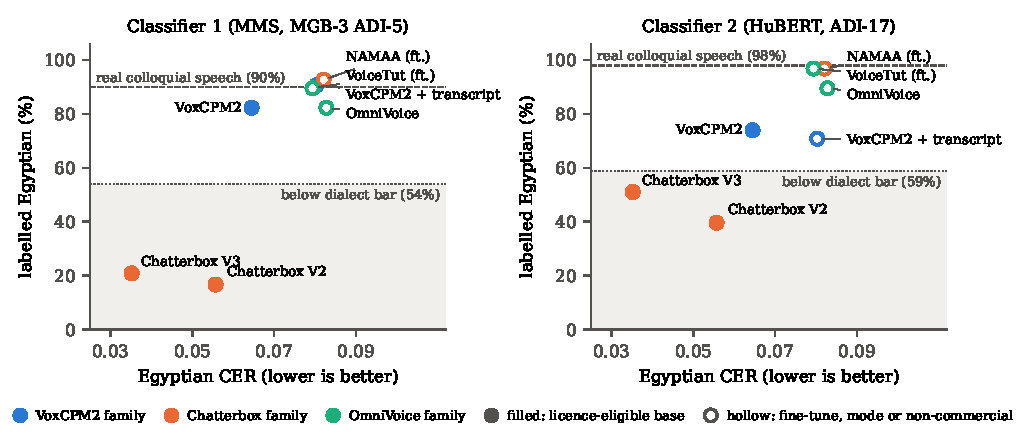
\includegraphics[width=\linewidth]{figures/dissociation.pdf}
\caption{Egyptian CER against the share of outputs labelled Egyptian, under two independent dialect classifiers
(bake-off, 96 utterances per system). Shaded: below the dialect bar, 60\% of the share on real colloquial speech. The
two lowest-CER systems are the two least Egyptian. Off the CER scale and not shown: \R{fig:offscale}.}
\label{fig:dissociation}
\end{figure}

\paragraph{Lowest CER, least Egyptian}
\cbthree has the lowest CER of all systems (\R{bk:cb-v3:cer}), and Chatterbox~V2 the second lowest
(\R{bk:cb-v2:cer}). Classifier~1 labels only \R{bk:cb-v3:c1pct} and \R{bk:cb-v2:c1pct} of their outputs Egyptian,
against \R{cal:lahgtna:c1pct} for real colloquial Egyptian speech; most of the rest is labelled Levantine
(\R{lab:cb-v3:Levantine} for V3), Gulf (\R{lab:cb-v3:Gulf}) or MSA (\R{lab:cb-v3:MSA}). \vox has a higher CER
(\R{bk:voxcpm2:cer}), with an interval that overlaps \cbthree's, and is labelled Egyptian \R{bk:voxcpm2:c1pct} of the
time. Speaker similarity and predicted quality do not separate the bases either: \cbthree has the highest DNSMOS of
the three eligible bases and Chatterbox~V2 the highest similarity.

\paragraph{What each metric would choose}
Point estimates on 96 utterances could pick a winner by chance, so we ask how often a selection rule fails, not
whether it failed once. We resample texts and voices (two-way bootstrap, \R{sel:B} resamples, the same draw for every
system), apply each rule in every resample, and record whether the chosen system clears the dialect bar in that
resample (\cref{tab:selection}). Among the three licence-eligible bases, the decision G1 actually had to make, every
standard metric picks a Chatterbox model: lowest CER picks \R{sel:eligible:cer:pick} in \R{sel:eligible:cer:pickshare}
of resamples, and the chosen system fails the bar in \R{sel:eligible:cer:fail1} of resamples under classifier~1 and
\R{sel:eligible:cer:fail2} under classifier~2; highest similarity fails in \R{sel:eligible:ecapa:fail1} and
\R{sel:eligible:ecapa:fail2}, highest predicted quality in \R{sel:eligible:dnsmos:fail1} and
\R{sel:eligible:dnsmos:fail2}. Lowest CER among the systems that clear the bar picks \vox in
\R{sel:eligible:amended:pickshare} of resamples. Across all nine configurations, which include Egyptian fine-tunes and
non-commercial models, lowest CER still fails the bar in \R{sel:all:cer:fail1} of resamples (classifier~1), while
highest similarity happens to pick OmniVoice, a non-commercial model that clears it. The failure is therefore not that
every metric always points away from the dialect, but that none of them carries information about it, so which system
they pick depends on what else is in the pool.

\begin{table}[t]
\centering\small
\caption{What each selection rule picks, over \R{sel:B} two-way bootstrap resamples of the bake-off (texts and voices
resampled, the same draw for every system). Pick: the rule's choice on the full data. Picked: share of resamples in
which the rule chose that system. Fails bar: share of resamples in which the rule's choice, whichever it was, falls
below the dialect bar (\R{sel:bar:c1} for classifier~1, \R{sel:bar:c2} for classifier~2). Last row: the amended G1.
$^\dagger$Non-commercial weights.}
\label{tab:selection}
\begin{adjustbox}{max width=\linewidth}
\rawinput{generated/tab_selection.tex}
\end{adjustbox}
\end{table}

\paragraph{Three seeds on held-out sentences}
The bake-off has one seed per utterance. On the 24 held-out Egyptian sentences, each generated with three seeds, the
paired comparison of \vox and \cbthree gives a CER difference of \R{pt:voxcpm2_minus_cb-v3:egy_main:cer_best:diff}
(95\% CI \R{pt:voxcpm2_minus_cb-v3:egy_main:cer_best:ci}) and a similarity difference of
\R{pt:voxcpm2_minus_cb-v3:egy_main:sim_ecapa:diff} (CI \R{pt:voxcpm2_minus_cb-v3:egy_main:sim_ecapa:ci}): the two
cannot be told apart. DNSMOS prefers \cbthree (\R{pt:voxcpm2_minus_cb-v3:egy_main:mos_p808:diff}, CI
\R{pt:voxcpm2_minus_cb-v3:egy_main:mos_p808:ci}). The Egyptian share separates them by
\R{pt:voxcpm2_minus_cb-v3:egy_main:c1:diff} under classifier~1 (CI \R{pt:voxcpm2_minus_cb-v3:egy_main:c1:ci},
$\R{pt:voxcpm2_minus_cb-v3:egy_main:c1:pholm}$) and \R{pt:voxcpm2_minus_cb-v3:egy_main:c2:diff} under classifier~2
(CI \R{pt:voxcpm2_minus_cb-v3:egy_main:c2:ci}, $\R{pt:voxcpm2_minus_cb-v3:egy_main:c2:pholm}$). With three seeds,
lowest CER picks \cbthree in \R{sel3:cer:cbv3} of resamples and highest DNSMOS in \R{sel3:dnsmos:cbv3}.

\paragraph{No relation across systems}
Across the nine configurations, Spearman's rank correlation between CER and the Egyptian share is
\R{sel:rhoc1} under classifier~1 (bootstrap 95\% interval \R{sel:rhoc1:ci}) and \R{sel:rhoc2} under classifier~2
(\R{sel:rhoc2:ci}). Nine systems cannot rule out a moderate relation in either direction, and we do not rest the claim
on these coefficients; the selection analysis above is the direct test.

\paragraph{Two classifiers, trained on different data, agree}
The finding could be an artefact of one classifier. Classifier~2 was trained on different speech (YouTube rather
than broadcast) with a different backbone and label set. It is more generous to every system, but it ranks the
systems in nearly the same order (Spearman $\rho=\R{rank:c1c2:rho}$, $p=\R{rank:c1c2:p}$), and under it too both
Chatterbox bases fall below the dialect bar while \vox clears it. Per utterance the classifiers agree moderately
(Cohen's $\kappa=\R{kappa:real}$ on calibration speech, \R{kappa:gen} on generated speech), so we rely on system-level
shares, not on single labels.

\paragraph{Not an artefact of the reference voices}
FLEURS references are read and mostly MSA in register, so a system could sound un-Egyptian because it copies the
reference's register. Splitting the bake-off by the dialect of the reference clip itself does not remove the gap under
classifier~1: with the \R{ref:egy:nvoices} references that both classifiers label Egyptian, \cbthree is labelled
Egyptian \R{ref:cb-v3:egy:c1} of the time and \vox \R{ref:voxcpm2:egy:c1}; with the \R{ref:msa:nvoices} references
labelled MSA by both, \R{ref:cb-v3:msa:c1} and \R{ref:voxcpm2:msa:c1}. Classifier~2 is more sensitive to the reference:
with Egyptian references it labels \cbthree Egyptian \R{ref:cb-v3:egy:c2} of the time against \R{ref:voxcpm2:egy:c2}
for \vox, a smaller gap than with MSA references (\R{ref:cb-v3:msa:c2} against \R{ref:voxcpm2:msa:c2}). Two or three
voices per group make these intervals wide (\texttt{selection.md}); the direction holds in every cell, but how much a
colloquial reference helps a model without Egyptian training data is a question for colloquial reference recordings
(\cref{sec:limitations}).

\paragraph{The ear agrees, informally}
In an informal check of six sentences per system, with names hidden and order shuffled, the author, a native Egyptian
speaker, rated both Chatterbox bases ``not Egyptian'' on \R{lt:cb-v3:not} sentences, and \vox ``not Egyptian'' on none
(Egyptian on \R{lt:voxcpm2:egy}, partly on \R{lt:voxcpm2:mid}). One listener who knew the hypothesis, rating six
sentences, settles nothing; we report the check because it agrees with both classifiers on the decision that matters,
and we do not count it as evidence on its own. A multi-listener test is the next step (\cref{sec:limitations}).

\paragraph{Why}
The pattern fits the training data rather than the architecture. The three Chatterbox-based systems without documented
Egyptian training data (V3, V2 and the lahgtna fine-tune) are labelled Levantine more than anything else
(\R{lab:chat:lev} of their outputs together), while NAMAA, a Chatterbox fine-tune on Egyptian speech, is labelled
Egyptian \R{bk:namaa:c1pct} of the time. A recogniser trained mostly on MSA and pan-Arabic data transcribes Levantine-
or MSA-accented Egyptian sentences correctly: the words survive, the dialect does not, and CER cannot see the
difference. Accent may even help CER, since speech closer to the recogniser's training distribution is easier to
transcribe. Our data cannot separate these explanations, but neither rescues CER as a selection criterion.

\paragraph{Consequence for model selection}
A selection rule that ranks by intelligibility, similarity or predicted quality, as our own pre-registered gate G1 did
with CER, picks a base without regard to the dialect. For any product whose purpose is to speak a dialect, these
metrics have to be paired with a dialect measure calibrated on real dialectal speech and, where possible, native
listeners, and the bar should be fixed relative to the same measure on real speech, since classifiers differ in how
generous they are.

\section{BA: an inference-time engine for Egyptian Arabic}\label{sec:engine}

\vox already clears every G3 bar for Egyptian Arabic, English and French, so the planned fine-tune was not needed to
list Egyptian, and no Egyptian training data with a licence and provenance we could accept exists beyond two
synthetic voices (NileTTS). \BA therefore keeps the \vox weights unchanged and adds an engine around them. Each
component targets a problem seen in the bake-off; each default was chosen on the tuning sentences only. The
ablations in \cref{sec:results} show which of them move the automatic metrics.

\paragraph{Egyptian number and symbol normaliser}
Digits were the largest error source for every system: on sentences with numbers, CER rose for all of them, and
the listening check noted that ``in most systems the number is not said the Egyptian way''. The normaliser writes
numbers as Cairenes say them, never in MSA: cardinals up to the billions, years, dates, times (\emph{7:30}
$\rightarrow$ \ar{sab3a-wnoss}), prices with currencies, percentages, decimals and simple fractions, phone numbers
digit by digit, ordinals, counted plurals (\emph{4 days} $\rightarrow$ \ar{arba3-ayyam}, with the Egyptian
counted form) and common symbols and abbreviations. Forms follow colloquial usage (\ar{khamastashar} ``fifteen'',
\ar{tultumiyya} ``three hundred''), not MSA (\ar{khamsata3ashar}, \ar{thalathumi2a}). English and French have
their own normalisers with the same coverage.

\paragraph{Loanword policy for code-switched text}
Egyptians mix English words into Arabic sentences. Left in Latin script, \vox reads them with English phonology;
written in Arabic script as Egyptians say them (\emph{meeting} $\rightarrow$ \ar{meeting}), they are read as part of
the Arabic sentence. \BA writes a list of common loanwords in Arabic script, spells short acronyms letter by letter
and leaves other Latin words as they are. On the tuning set this kept intelligibility level (canonical-script CER
\R{cs:keep:cer} kept vs \R{cs:arabic:cer} transliterated) and raised the Egyptian share from \R{cs:keep:c1pct} to
\R{cs:arabic:c1pct}.

\paragraph{Reference transcript}
\vox can condition on the reference audio alone or on the audio and its transcript. In the bake-off the transcript
raised speaker similarity from \R{bk:voxcpm2:ecapa} to \R{bk:voxcpm2-prompt:ecapa} and the Egyptian share from
\R{bk:voxcpm2:c1pct} to \R{bk:voxcpm2-prompt:c1pct}. Users rarely type what they said, so \BA transcribes the
reference with Whisper large-v3-turbo \citep{openai2024whisperturbo}, which on real colloquial Egyptian speech is
close to large-v3 (\R{asr:turbo:cer} vs \R{asr:large:cer} CER) at a fraction of the cost.

\paragraph{Reference preparation}
Uploads are converted to mono 16\,kHz, screened, and cut to the cleanest 6--15\,s window: long pauses are shortened
and the level is normalised. A recording is rejected, with a message the user can act on, if it is too short, too
noisy or clipped. The noise and clipping thresholds were set midway between the worst clean and the best degraded
references in a controlled test, and reject none of the \R{ref:clean:n} real clean clips we checked.

\paragraph{Long text}
\vox degrades on long inputs. \BA splits text into sentences, packs them into chunks of at most
\R{chunk:maxchars} characters without breaking a sentence, generates each chunk, checks its speaking rate and level
against the bands measured on real speech, retries a failing chunk up to twice with a new seed, and joins the chunks
with pauses that depend on the punctuation.

\paragraph{Generation settings and watermark}
Classifier-free guidance 2.0 and 10 diffusion steps, chosen by a six-setting sweep on the tuning sentences. Every
output is watermarked with AudioSeal \citep{sanroman2024audioseal} with a fixed 16-bit message: the mark is computed on
a 16\,kHz copy and added to the 48\,kHz output, leaving content above 8\,kHz untouched (\cref{sec:release}).

\paragraph{What \BA does not change}
No weights are modified. Any gain over \vox therefore comes from what the model is given (text, reference, transcript)
and how its output is checked, which the ablations in \cref{sec:results} separate.

\section{Results}\label{sec:results}

All engine results are on held-out sentences (\cref{sec:protocol}) with the bake-off's voices. ``\vox (plain)'' is
the same model driven directly with the reference audio, as in the bake-off.

\subsection{\BA against the base model and the Egyptian baselines}

\begin{table}[t]
\centering\small
\caption{Held-out Egyptian sentences over \R{s3:nseeds} seeds per utterance (mean and two-way bootstrap 95\% interval over
texts and voices; seeds of one utterance are kept together). NAMAA is the best Egyptian fine-tune with permissive
weights; Chatterbox V3 is the lowest-CER system of the bake-off.}
\label{tab:seeds}
\begin{adjustbox}{max width=\linewidth}
\rawinput{generated/tab_seeds.tex}
\end{adjustbox}
\end{table}

\Cref{tab:seeds} compares \BA with \vox (plain), NAMAA and \cbthree. Against its own base, \BA lowers Egyptian CER
from \R{s3:voxcpm2:egy_main:cer_best} to \R{s3:ba:egy_main:cer_best}
(paired difference \R{pt:ba_minus_voxcpm2:egy_main:cer_best:diff}, 95\% CI \R{pt:ba_minus_voxcpm2:egy_main:cer_best:ci},
$\R{pt:ba_minus_voxcpm2:egy_main:cer_best:pholm}$) and raises speaker similarity from
\R{s3:voxcpm2:egy_main:sim_ecapa} to \R{s3:ba:egy_main:sim_ecapa}
(\R{pt:ba_minus_voxcpm2:egy_main:sim_ecapa:diff}, CI \R{pt:ba_minus_voxcpm2:egy_main:sim_ecapa:ci},
$\R{pt:ba_minus_voxcpm2:egy_main:sim_ecapa:pholm}$). The Egyptian share also rises
(\R{pt:ba_minus_voxcpm2:egy_main:c1:diff} under classifier~1), but its interval includes zero
(\R{pt:ba_minus_voxcpm2:egy_main:c1:ci}); with three voices per condition, a difference of this size cannot be
resolved, and we do not claim it. \BA matches \cbthree on CER
(\R{pt:ba_minus_cb-v3:egy_main:cer_best:diff}, CI \R{pt:ba_minus_cb-v3:egy_main:cer_best:ci}) while being labelled
Egyptian far more often (\R{pt:ba_minus_cb-v3:egy_main:c1:diff}, CI \R{pt:ba_minus_cb-v3:egy_main:c1:ci}). In short,
\BA has the intelligibility of the lowest-CER system and the dialect of the Egyptian ones, with the highest speaker
similarity of the four. Predicted quality (DNSMOS) favours \cbthree
(\R{pt:ba_minus_cb-v3:egy_main:mos_p808:diff}, CI \R{pt:ba_minus_cb-v3:egy_main:mos_p808:ci}), as it does over \vox;
as an English-trained predictor it is a weak signal for Arabic \citep{kunesova2024zeroshotmos}, and its preference for
the least Egyptian system is one more instance of the blind spot in \cref{sec:dissociation}. \BA raises DNSMOS over
its own base (\R{pt:ba_minus_voxcpm2:egy_main:mos_p808:diff}, CI \R{pt:ba_minus_voxcpm2:egy_main:mos_p808:ci}).

\paragraph{Numbers}
On held-out sentences with digits, scored against the best of the spelled-out Egyptian form and the digit text,
\BA's CER is \R{s3:ba:egy_digits:cer_best} against \R{s3:voxcpm2:egy_digits:cer_best} for \vox (plain). CER here
understates the normaliser's effect, because a recogniser can transcribe an MSA reading of a number into the same
digits; whether the number \emph{sounds} Egyptian is a question for listeners (\cref{sec:limitations}).

\subsection{Ablations: where the gain comes from}

\begin{table}[t]
\centering\small
\caption{Ablations on held-out sentences (seed index 0, same utterances in every row). Each middle row removes one
component from \BA; the last row is \vox used directly. Bold: the paired 95\% interval of the difference from full
\BA excludes zero. CER$_\text{canon.}$: CER after mapping Latin and Arabic-script spellings of the same loanword to
one form. Egy.: share labelled Egyptian by classifier~1. Intervals for every cell are in \texttt{ablations.md}.}
\label{tab:ablation}
\begin{adjustbox}{max width=\linewidth}
\rawinput{generated/tab_ablation.tex}
\end{adjustbox}
\end{table}

\Cref{tab:ablation} removes one component at a time. One component carries almost all of the measurable gain: the
automatic reference transcript. Without it, Egyptian CER rises from \R{ab:full:egy_main:err} to
\R{ab:no_transcript:egy_main:err} (the paired interval includes zero), speaker similarity changes by
\R{ab:no_transcript:egy_main:sim_ecapa:diff} (CI \R{ab:no_transcript:egy_main:sim_ecapa:ci}), and on code-switched
sentences the Egyptian share falls from \R{ab:full:cs:c1} to \R{ab:no_transcript:cs:c1} while CER rises; in English,
similarity changes by \R{ab:no_transcript:en:sim_ecapa:diff}. Removing it accounts for about \R{ab:share:notrans:ecapa}
of \BA's similarity gain over \vox (plain) and \R{ab:share:notrans:cer} of its CER gain on Egyptian sentences.

The other components leave the automatic metrics unchanged. Reference preparation makes no measurable difference on
FLEURS references, which are already clean studio-quality clips; its job is to reject or repair the phone recordings
of real users, which this test set does not contain. The chunk check never triggered (\R{ab:chunk:retries} retries
in 150 utterances), so removing it would reproduce full \BA. Most telling for this paper, the Egyptian number
normaliser does not change CER on digit sentences (\R{ab:full:egy_digits:err} with it, \R{ab:no_normaliser:egy_digits:err}
without) and the loanword policy does not change canonical CER. Both change \emph{what is said}: without the
normaliser, \vox reads \emph{7:30} or \emph{15} as it sees fit (the bake-off listening check found that most systems did
not say numbers the Egyptian way), and the recogniser writes any reading back as the same digits. The metric that cannot see a dialect cannot see a dialectal number either. Whether
these components make the speech sound more Egyptian is a question for listeners, and we leave it to the listening
test rather than claim it.
\subsection{English, French and cross-language cloning}
All three languages pass G3 on held-out sentences. In English, \BA's WER is \R{ho:ba:en:wer} with no failures
(\R{ho:ba:en:fail}), and speaker similarity rises from \R{ho:voxcpm2:en:ecapa} for \vox (plain), below the G3 bar of
\R{g3:en:simbar}, to \R{ho:ba:en:ecapa}; plain \vox also produced empty outputs on \R{ho:voxcpm2:en:fail} English
sentences. In French, WER is \R{ho:ba:fr:wer} and similarity \R{ho:ba:fr:ecapa} (bar \R{g3:fr:simbar}). When an
Egyptian voice speaks English or French, similarity is \R{xl:cross_en:ba} and \R{xl:cross_fr:ba} for \BA against
\R{xl:cross_en:raw} and \R{xl:cross_fr:raw} for \vox (plain); the French figure sits at 80\% of the Egyptian
same-speaker ceiling, and the model card lists cross-language use as a limitation.

\subsection{Long text}
\Cref{tab:long} gives the 24 long passages written after the engine was frozen (8 per language, each in two voices,
\R{lf:ba:arz:audio_sec}\,s of Egyptian audio on average). Neither system failed on any passage, so this test does not
show the benefit of \BA's chunk checks that motivated them: \BA split Egyptian passages into
\R{lf:ba:arz:chunks} chunks on average (at most \R{chunk:maxchars} characters each) and no chunk needed a retry
(\R{lf:ba:retries} retries in all). Speaker similarity is higher with \BA in
all three languages (Egyptian \R{lfp:arz:sim_ecapa:diff}, CI \R{lfp:arz:sim_ecapa:ci}; English
\R{lfp:en:sim_ecapa:diff}, CI \R{lfp:en:sim_ecapa:ci}; French \R{lfp:fr:sim_ecapa:diff}, CI \R{lfp:fr:sim_ecapa:ci}),
as on short sentences. Error rates do not separate the systems, and they expose a measurement problem for long
synthetic Egyptian speech. Whisper's sequential long-form decoding fell into a repetition loop over the first 25\,s of
one \BA passage and returned one word about a hundred times (CER \R{lfw:clip:ba:arz02:seq}); transcribing the same
audio in pieces returns the passage. Re-scoring every long clip of both systems in $\sim$20\,s windows cut at pauses
repairs that clip (\R{lfw:clip:ba:arz02:win}) but breaks another passage for both systems, where Whisper rewrites the
colloquial opening into MSA and then loops (CER \R{lfw:clip:ba:arz05:win} for \BA and
\R{lfw:clip:voxcpm2:arz05:win} for \vox). The Egyptian CER difference between \BA and \vox is
\R{lfp:arz:err:diff} (CI \R{lfp:arz:err:ci}) under sequential decoding and \R{lfwp:arz:err_win:diff}
(CI \R{lfwp:arz:err_win:ci}) under windowed decoding; we draw no conclusion about long-form Egyptian CER from either.
Scoring long synthetic speech with Whisper needs loop detection or a second recogniser, and the rewriting of Egyptian
into MSA is the blind spot of \cref{sec:dissociation} inside the recogniser itself.

\begin{table}[t]
\centering\small
\caption{Long passages written after the engine was frozen (8 per language $\times$ 2 voices; one seed). Means with
two-way bootstrap 95\% intervals. Sequential ASR is the protocol's metric; windowed ASR transcribes $\sim$20\,s pieces
cut at pauses and is a secondary analysis. Egyptian: share labelled Egyptian by classifier~1.}
\label{tab:long}
\begin{adjustbox}{max width=\linewidth}
\rawinput{generated/tab_long.tex}
\end{adjustbox}
\end{table}

\subsection{Speed and memory}
On one NVIDIA A40, \BA loads in \R{bench:load}\,s, prepares a voice from a 10\,s recording in \R{bench:voice}\,s, and
speaks a \R{bench:arz:words}-word Egyptian sentence (\R{bench:arz:audio}\,s of audio) in \R{bench:arz:time}\,s and a
\R{bench:arzlong:words}-word passage (\R{bench:arzlong:audio}\,s) in \R{bench:arzlong:time}\,s, with a peak of
\R{bench:vram}\,GB of GPU memory. On two CPU threads \vox runs about \R{bk:voxcpm2:cpurtf} times slower than real
time, so the public demo needs a GPU.

\section{A consent-first release}\label{sec:release}

A voice is personal data, and a cloning system can be used to impersonate people
\citep{hutiri2024notmyvoice}. \BA's release follows from that.

\paragraph{What is published}
The engine (code and text normalisers), its configuration, the evaluation texts, per-utterance scores and all
scripts are public. The model repository serves the unchanged \vox weights with \BA's configuration and package; the
demo runs the same code. \BA's own work is under a non-commercial community licence with conditions against
impersonation and use without consent; \vox and the other components keep their own licences (Apache-2.0 and MIT),
which allow a derivative to carry stricter terms. The licence has not been reviewed by a lawyer, and we say so.

\paragraph{What is not published}
No FLEURS speaker's audio or clone is redistributed: those speakers licensed recordings for speech research, not
public demonstrations of their cloned voices saying new things. Samples on the model card clone two synthetic
Egyptian voices designed from a text description with \vox.

\paragraph{Consent and storage}
The demo does not generate until the user confirms, in Arabic and English, that the voice is theirs or that they
have the speaker's explicit permission. Uploads are copied to a per-request temporary directory that is deleted when
the request ends; the prepared voice lives only in the browser session's memory; no text or audio is logged, and
analytics are off.

\paragraph{Watermark}
Every output carries an AudioSeal watermark with a fixed 16-bit message. In a first check, it was detected in all
\R{wm:ba:n} held-out \BA outputs as WAV, as MP3 at 128 and 64\,kbit/s and after resampling to 16\,kHz, and in none
of the \R{wm:clean:n} unwatermarked clips (plain \vox outputs and real speech).
\pending{Robustness under 25 attacks (noise and babble at 20/10/5\,dB, speed and tempo changes, telephone band,
MP3/AAC/Opus at low bit rates and chains of them, 3-second excerpts, gain and loudness changes), with detection and
false-positive rates, from watermark\_attacks.py.} A watermark helps platforms and investigators identify \BA output;
it does not stop someone who strips it or uses another system, and we do not present it as a safeguard on its own.

\section{Limitations}\label{sec:limitations}

\paragraph{Human judgement}
The listening evidence is one native listener, the author, rating six sentences per system blind. It agrees with two
classifiers on the decision that matters, but it is not a listening test. A blind test with multiple native Egyptian
listeners rating naturalness, Egyptian authenticity, similarity and correctness, with real speech as a hidden
anchor, is the next step \pending{and will be reported in a revision}.

\paragraph{Reference voices}
FLEURS speakers read prepared text, mostly in an MSA register; only some of their clips are labelled Egyptian by the
classifiers. Cloning colloquial Egyptian from such references is harder than from everyday speech, and our numbers
may understate what all systems do with a colloquial reference. Six Egyptian voices, three per sentence, also make
the intervals wide.

\paragraph{Classifiers as dialect measures}
Both classifiers label real colloquial Egyptian speech as Egyptian most of the time, but they are trained on
broadcast and online speech, not on synthetic speech, and they disagree on many single utterances. We therefore use
system-level shares, calibrate the bar on real speech, and report both classifiers.

\paragraph{Scope}
\BA adds no training; dialect features that \vox cannot produce, \BA cannot add. Results are for Egyptian Arabic,
English and French with the systems available in November 2026. The text normaliser covers Cairene usage; other
Egyptian varieties (for example Upper Egyptian) are not covered.

\paragraph{Misuse}
Despite the consent step and the watermark, a determined user can clone a voice without permission. We release
because the same technology is already public in less careful forms, and because an open, measured Egyptian system
helps people build, audit and detect such systems; this is a judgement, not a guarantee.

\section{Conclusion}\label{sec:conclusion}

For Egyptian Arabic voice cloning, the metric that a practitioner would reach for first, intelligibility, selects
the wrong model: the open system with the lowest character error rate was the least Egyptian, by two independent
classifiers and by ear, and our own selection rule would have chosen it. A protocol that pairs intelligibility with
a dialect bar calibrated on real colloquial speech selects a different base, on which \BA, an inference-time engine
for Egyptian text, references and long inputs, reaches the intelligibility of the best system while keeping the
dialect, with no new training. For any dialect, we recommend that evaluations report a calibrated dialect measure
next to error rates, and that selection rules state the dialect bar before the first model is run.

\section*{Declaration of competing interest}
The author declares no competing financial interests or personal relationships that could have appeared to
influence the work reported in this paper.

\section*{Funding}
This research did not receive any specific grant from funding agencies in the public, commercial, or not-for-profit
sectors.

\section*{Data and code availability}
The code, evaluation texts, per-utterance scores and the scripts that produce every number, table and figure are
archived with the paper sources on Zenodo (\zenodo); the engine source also ships with the demo. The model is at \hfmodel and the demo at \hfspace. FLEURS \citep{conneau2023fleurs}, lahgtna-v2 \citep{oddadmix2026lahgtnadata}
and NileTTS \citep{khamis2026niletts} are public datasets; FLEURS reference clips and the audio cloned from them are not
redistributed (\cref{sec:release}).

\section*{Ethics}
\emph{Listening test.} Native Egyptian adults took part in the blind listening test (\cref{sec:dissociation},
\cref{app:listening}) as unpaid volunteers. The first page of the test stated the purpose of the study, that taking part was
voluntary and could be stopped at any time by closing the page, what would be stored, and that the results would be
published only in aggregate, and it gave a contact address; listeners confirmed that they were 18 or older and agreed to
take part before the first clip. The test asked for no name or contact details and its database stored no IP address:
each session holds a random identifier, the ratings and four coarse descriptors (age band, gender, governorate,
listening device). Individual answers are not published. Listeners heard speech cloned from FLEURS speakers, released for
speech research, and real clips from the public lahgtna-v2 corpus; they were asked not to record or share the clips, and
no new recordings of people were made. No institutional ethics review was sought: taking part was anonymous, voluntary and unpaid, consisted only of listening to short clips and rating them, carried no foreseeable risk beyond those of everyday life, and collected no information that identifies a person.

\emph{Voice cloning.} Voice cloning can impersonate people. The safeguards of the release (a consent statement in the
demo, no storage of uploads, an AudioSeal watermark on every output) and their limits are described in
\cref{sec:release}.

\section*{Declaration of generative AI and AI-assisted technologies in the manuscript preparation process}
During the preparation of this work, the author used Claude (Anthropic) for help with code and with the academic
writing. After using this tool, the author reviewed and edited the content as needed and takes full responsibility for
the content of the published article.


\bibliographystyle{elsarticle-num-names}
\bibliography{refs}

\appendix
\section{Additional tables}\label{app:tables}

\pending{Full bake-off tables for every condition (Egyptian, digits, diacritised, code-switched, English, French,
cross-language, long passages) with failure counts and speed, generated from bakeoff.json and
dialect\_classifier2.json; reference clips and their dialect labels; Chatterbox V3 under the two loaders.}

\section{Claim-to-results map}\label{app:claims}

Every number in the paper is produced by \texttt{BA/paper/scripts/make\_assets.py} from the files below, each of which
records the command that produced it.

\begin{center}\small
\begin{tabular}{@{}ll@{}}
\toprule
Section & Results files (\texttt{BA/eval/results/}) \\
\midrule
\Cref{sec:protocol} (calibration) & \texttt{bakeoff.json}, \texttt{dialect\_classifier2.json} \\
\Cref{sec:dissociation} & \texttt{bakeoff.json}, \texttt{bakeoff\_utterances.csv}, \texttt{dialect\_classifier2.json}, \texttt{listening\_test.json} \\
\Cref{sec:engine} & \texttt{codeswitch\_policy.json}, \texttt{asr\_check.json}, \texttt{chunk\_length.json}, \texttt{reference\_thresholds.json}, \texttt{engine.json} \\
\Cref{sec:results} & \texttt{uncertainty.json}, \texttt{ablations.json}, \texttt{engine.json}, \texttt{bench.json} \\
\Cref{sec:release} & \texttt{watermark.json}, \texttt{watermark\_attacks.json} \\
\bottomrule
\end{tabular}
\end{center}

\end{document}
